\documentclass[a4paper, 11pt]{book}

    \usepackage[breakable]{tcolorbox}
    \usepackage{parskip} 
    % Stop auto-indenting (to mimic markdown behaviour)    
    % Basic figure setup, for now with no caption control since it's done
    % automatically by Pandoc (which extracts ![](path) syntax from Markdown).
    \usepackage{graphicx}
    % Keep aspect ratio if custom image width or height is specified
    \setkeys{Gin}{keepaspectratio}
    % Maintain compatibility with old templates. Remove in nbconvert 6.0
    \let\Oldincludegraphics\includegraphics
    % Ensure that by default, figures have no caption (until we provide a
    % proper Figure object with a Caption API and a way to capture that
    % in the conversion process - todo).
    \usepackage{caption}
    \DeclareCaptionFormat{nocaption}{}
    \captionsetup{format=nocaption,aboveskip=0pt,belowskip=0pt}

    \usepackage{float}
    \floatplacement{figure}{H} % forces figures to be placed at the correct location
    \usepackage{xcolor} % Allow colors to be defined
    \usepackage{enumerate} % Needed for markdown enumerations to work
    \usepackage{geometry} % Used to adjust the document margins
    \usepackage{amsmath} % Equations
    \usepackage{amssymb} % Equations
    \usepackage{textcomp} % defines textquotesingle
    % Hack from http://tex.stackexchange.com/a/47451/13684:
    \AtBeginDocument{%
        \def\PYZsq{\textquotesingle}% Upright quotes in Pygmentized code
    }
    \usepackage{upquote} % Upright quotes for verbatim code
    \usepackage{eurosym} % defines \euro

    \usepackage{iftex}
    \ifPDFTeX
        \usepackage[T1]{fontenc}
        \IfFileExists{alphabeta.sty}{
              \usepackage{alphabeta}
          }{
              \usepackage[mathletters]{ucs}
              \usepackage[utf8x]{inputenc}
          }
    \else
        \usepackage{fontspec}
        \usepackage{unicode-math}
    \fi

    \usepackage{fancyvrb} % verbatim replacement that allows latex
    \usepackage{grffile} % extends the file name processing of package graphics
                         % to support a larger range
    \makeatletter % fix for old versions of grffile with XeLaTeX
    \@ifpackagelater{grffile}{2019/11/01}
    {
      % Do nothing on new versions
    }
    {
      \def\Gread@@xetex#1{%
        \IfFileExists{"\Gin@base".bb}%
        {\Gread@eps{\Gin@base.bb}}%
        {\Gread@@xetex@aux#1}%
      }
    }
    \makeatother
    \usepackage[Export]{adjustbox} % Used to constrain images to a maximum size
    \adjustboxset{max size={0.9\linewidth}{0.9\paperheight}}

    % The hyperref package gives us a pdf with properly built
    % internal navigation ('pdf bookmarks' for the table of contents,
    % internal cross-reference links, web links for URLs, etc.)
    \usepackage{hyperref}
    % The default LaTeX title has an obnoxious amount of whitespace. By default,
    % titling removes some of it. It also provides customization options.
    \usepackage{titling}
    \usepackage{longtable} % longtable support required by pandoc >1.10
    \usepackage{booktabs}  % table support for pandoc > 1.12.2
    \usepackage{array}     % table support for pandoc >= 2.11.3
    \usepackage{calc}      % table minipage width calculation for pandoc >= 2.11.1
    \usepackage[inline]{enumitem} % IRkernel/repr support (it uses the enumerate* environment)
    \usepackage[normalem]{ulem} % ulem is needed to support strikethroughs (\sout)
                                % normalem makes italics be italics, not underlines
    \usepackage{soul}      % strikethrough (\st) support for pandoc >= 3.0.0
    \usepackage{mathrsfs}
    

    
    % Colors for the hyperref package
    \definecolor{urlcolor}{rgb}{0,.145,.698}
    \definecolor{linkcolor}{rgb}{.71,0.21,0.01}
    \definecolor{citecolor}{rgb}{.12,.54,.11}

    % ANSI colors
    \definecolor{ansi-black}{HTML}{3E424D}
    \definecolor{ansi-black-intense}{HTML}{282C36}
    \definecolor{ansi-red}{HTML}{E75C58}
    \definecolor{ansi-red-intense}{HTML}{B22B31}
    \definecolor{ansi-green}{HTML}{00A250}
    \definecolor{ansi-green-intense}{HTML}{007427}
    \definecolor{ansi-yellow}{HTML}{DDB62B}
    \definecolor{ansi-yellow-intense}{HTML}{B27D12}
    \definecolor{ansi-blue}{HTML}{208FFB}
    \definecolor{ansi-blue-intense}{HTML}{0065CA}
    \definecolor{ansi-magenta}{HTML}{D160C4}
    \definecolor{ansi-magenta-intense}{HTML}{A03196}
    \definecolor{ansi-cyan}{HTML}{60C6C8}
    \definecolor{ansi-cyan-intense}{HTML}{258F8F}
    \definecolor{ansi-white}{HTML}{C5C1B4}
    \definecolor{ansi-white-intense}{HTML}{A1A6B2}
    \definecolor{ansi-default-inverse-fg}{HTML}{FFFFFF}
    \definecolor{ansi-default-inverse-bg}{HTML}{000000}

    % common color for the border for error outputs.
    \definecolor{outerrorbackground}{HTML}{FFDFDF}

    % commands and environments needed by pandoc snippets
    % extracted from the output of `pandoc -s`
    \providecommand{\tightlist}{%
      \setlength{\itemsep}{0pt}\setlength{\parskip}{0pt}}
    \DefineVerbatimEnvironment{Highlighting}{Verbatim}{commandchars=\\\{\}}
    % Add ',fontsize=\small' for more characters per line
    \newenvironment{Shaded}{}{}
    \newcommand{\KeywordTok}[1]{\textcolor[rgb]{0.00,0.44,0.13}{\textbf{{#1}}}}
    \newcommand{\DataTypeTok}[1]{\textcolor[rgb]{0.56,0.13,0.00}{{#1}}}
    \newcommand{\DecValTok}[1]{\textcolor[rgb]{0.25,0.63,0.44}{{#1}}}
    \newcommand{\BaseNTok}[1]{\textcolor[rgb]{0.25,0.63,0.44}{{#1}}}
    \newcommand{\FloatTok}[1]{\textcolor[rgb]{0.25,0.63,0.44}{{#1}}}
    \newcommand{\CharTok}[1]{\textcolor[rgb]{0.25,0.44,0.63}{{#1}}}
    \newcommand{\StringTok}[1]{\textcolor[rgb]{0.25,0.44,0.63}{{#1}}}
    \newcommand{\CommentTok}[1]{\textcolor[rgb]{0.38,0.63,0.69}{\textit{{#1}}}}
    \newcommand{\OtherTok}[1]{\textcolor[rgb]{0.00,0.44,0.13}{{#1}}}
    \newcommand{\AlertTok}[1]{\textcolor[rgb]{1.00,0.00,0.00}{\textbf{{#1}}}}
    \newcommand{\FunctionTok}[1]{\textcolor[rgb]{0.02,0.16,0.49}{{#1}}}
    \newcommand{\RegionMarkerTok}[1]{{#1}}
    \newcommand{\ErrorTok}[1]{\textcolor[rgb]{1.00,0.00,0.00}{\textbf{{#1}}}}
    \newcommand{\NormalTok}[1]{{#1}}

    % Additional commands for more recent versions of Pandoc
    \newcommand{\ConstantTok}[1]{\textcolor[rgb]{0.53,0.00,0.00}{{#1}}}
    \newcommand{\SpecialCharTok}[1]{\textcolor[rgb]{0.25,0.44,0.63}{{#1}}}
    \newcommand{\VerbatimStringTok}[1]{\textcolor[rgb]{0.25,0.44,0.63}{{#1}}}
    \newcommand{\SpecialStringTok}[1]{\textcolor[rgb]{0.73,0.40,0.53}{{#1}}}
    \newcommand{\ImportTok}[1]{{#1}}
    \newcommand{\DocumentationTok}[1]{\textcolor[rgb]{0.73,0.13,0.13}{\textit{{#1}}}}
    \newcommand{\AnnotationTok}[1]{\textcolor[rgb]{0.38,0.63,0.69}{\textbf{\textit{{#1}}}}}
    \newcommand{\CommentVarTok}[1]{\textcolor[rgb]{0.38,0.63,0.69}{\textbf{\textit{{#1}}}}}
    \newcommand{\VariableTok}[1]{\textcolor[rgb]{0.10,0.09,0.49}{{#1}}}
    \newcommand{\ControlFlowTok}[1]{\textcolor[rgb]{0.00,0.44,0.13}{\textbf{{#1}}}}
    \newcommand{\OperatorTok}[1]{\textcolor[rgb]{0.40,0.40,0.40}{{#1}}}
    \newcommand{\BuiltInTok}[1]{{#1}}
    \newcommand{\ExtensionTok}[1]{{#1}}
    \newcommand{\PreprocessorTok}[1]{\textcolor[rgb]{0.74,0.48,0.00}{{#1}}}
    \newcommand{\AttributeTok}[1]{\textcolor[rgb]{0.49,0.56,0.16}{{#1}}}
    \newcommand{\InformationTok}[1]{\textcolor[rgb]{0.38,0.63,0.69}{\textbf{\textit{{#1}}}}}
    \newcommand{\WarningTok}[1]{\textcolor[rgb]{0.38,0.63,0.69}{\textbf{\textit{{#1}}}}}
    \makeatletter
    \newsavebox\pandoc@box
    \newcommand*\pandocbounded[1]{%
      \sbox\pandoc@box{#1}%
      % scaling factors for width and height
      \Gscale@div\@tempa\textheight{\dimexpr\ht\pandoc@box+\dp\pandoc@box\relax}%
      \Gscale@div\@tempb\linewidth{\wd\pandoc@box}%
      % select the smaller of both
      \ifdim\@tempb\p@<\@tempa\p@
        \let\@tempa\@tempb
      \fi
      % scaling accordingly (\@tempa < 1)
      \ifdim\@tempa\p@<\p@
        \scalebox{\@tempa}{\usebox\pandoc@box}%
      % scaling not needed, use as it is
      \else
        \usebox{\pandoc@box}%
      \fi
    }
    \makeatother

    % Define a nice break command that doesn't care if a line doesn't already
    % exist.
    \def\br{\hspace*{\fill} \\* }
    % Math Jax compatibility definitions
    \def\gt{>}
    \def\lt{<}
    \let\Oldtex\TeX
    \let\Oldlatex\LaTeX
    \renewcommand{\TeX}{\textrm{\Oldtex}}
    \renewcommand{\LaTeX}{\textrm{\Oldlatex}}
    % Document parameters
        
% Pygments definitions
\makeatletter
\def\PY@reset{\let\PY@it=\relax \let\PY@bf=\relax%
    \let\PY@ul=\relax \let\PY@tc=\relax%
    \let\PY@bc=\relax \let\PY@ff=\relax}
\def\PY@tok#1{\csname PY@tok@#1\endcsname}
\def\PY@toks#1+{\ifx\relax#1\empty\else%
    \PY@tok{#1}\expandafter\PY@toks\fi}
\def\PY@do#1{\PY@bc{\PY@tc{\PY@ul{%
    \PY@it{\PY@bf{\PY@ff{#1}}}}}}}
\def\PY#1#2{\PY@reset\PY@toks#1+\relax+\PY@do{#2}}

\@namedef{PY@tok@w}{\def\PY@tc##1{\textcolor[rgb]{0.73,0.73,0.73}{##1}}}
\@namedef{PY@tok@c}{\let\PY@it=\textit\def\PY@tc##1{\textcolor[rgb]{0.24,0.48,0.48}{##1}}}
\@namedef{PY@tok@cp}{\def\PY@tc##1{\textcolor[rgb]{0.61,0.40,0.00}{##1}}}
\@namedef{PY@tok@k}{\let\PY@bf=\textbf\def\PY@tc##1{\textcolor[rgb]{0.00,0.50,0.00}{##1}}}
\@namedef{PY@tok@kp}{\def\PY@tc##1{\textcolor[rgb]{0.00,0.50,0.00}{##1}}}
\@namedef{PY@tok@kt}{\def\PY@tc##1{\textcolor[rgb]{0.69,0.00,0.25}{##1}}}
\@namedef{PY@tok@o}{\def\PY@tc##1{\textcolor[rgb]{0.40,0.40,0.40}{##1}}}
\@namedef{PY@tok@ow}{\let\PY@bf=\textbf\def\PY@tc##1{\textcolor[rgb]{0.67,0.13,1.00}{##1}}}
\@namedef{PY@tok@nb}{\def\PY@tc##1{\textcolor[rgb]{0.00,0.50,0.00}{##1}}}
\@namedef{PY@tok@nf}{\def\PY@tc##1{\textcolor[rgb]{0.00,0.00,1.00}{##1}}}
\@namedef{PY@tok@nc}{\let\PY@bf=\textbf\def\PY@tc##1{\textcolor[rgb]{0.00,0.00,1.00}{##1}}}
\@namedef{PY@tok@nn}{\let\PY@bf=\textbf\def\PY@tc##1{\textcolor[rgb]{0.00,0.00,1.00}{##1}}}
\@namedef{PY@tok@ne}{\let\PY@bf=\textbf\def\PY@tc##1{\textcolor[rgb]{0.80,0.25,0.22}{##1}}}
\@namedef{PY@tok@nv}{\def\PY@tc##1{\textcolor[rgb]{0.10,0.09,0.49}{##1}}}
\@namedef{PY@tok@no}{\def\PY@tc##1{\textcolor[rgb]{0.53,0.00,0.00}{##1}}}
\@namedef{PY@tok@nl}{\def\PY@tc##1{\textcolor[rgb]{0.46,0.46,0.00}{##1}}}
\@namedef{PY@tok@ni}{\let\PY@bf=\textbf\def\PY@tc##1{\textcolor[rgb]{0.44,0.44,0.44}{##1}}}
\@namedef{PY@tok@na}{\def\PY@tc##1{\textcolor[rgb]{0.41,0.47,0.13}{##1}}}
\@namedef{PY@tok@nt}{\let\PY@bf=\textbf\def\PY@tc##1{\textcolor[rgb]{0.00,0.50,0.00}{##1}}}
\@namedef{PY@tok@nd}{\def\PY@tc##1{\textcolor[rgb]{0.67,0.13,1.00}{##1}}}
\@namedef{PY@tok@s}{\def\PY@tc##1{\textcolor[rgb]{0.73,0.13,0.13}{##1}}}
\@namedef{PY@tok@sd}{\let\PY@it=\textit\def\PY@tc##1{\textcolor[rgb]{0.73,0.13,0.13}{##1}}}
\@namedef{PY@tok@si}{\let\PY@bf=\textbf\def\PY@tc##1{\textcolor[rgb]{0.64,0.35,0.47}{##1}}}
\@namedef{PY@tok@se}{\let\PY@bf=\textbf\def\PY@tc##1{\textcolor[rgb]{0.67,0.36,0.12}{##1}}}
\@namedef{PY@tok@sr}{\def\PY@tc##1{\textcolor[rgb]{0.64,0.35,0.47}{##1}}}
\@namedef{PY@tok@ss}{\def\PY@tc##1{\textcolor[rgb]{0.10,0.09,0.49}{##1}}}
\@namedef{PY@tok@sx}{\def\PY@tc##1{\textcolor[rgb]{0.00,0.50,0.00}{##1}}}
\@namedef{PY@tok@m}{\def\PY@tc##1{\textcolor[rgb]{0.40,0.40,0.40}{##1}}}
\@namedef{PY@tok@gh}{\let\PY@bf=\textbf\def\PY@tc##1{\textcolor[rgb]{0.00,0.00,0.50}{##1}}}
\@namedef{PY@tok@gu}{\let\PY@bf=\textbf\def\PY@tc##1{\textcolor[rgb]{0.50,0.00,0.50}{##1}}}
\@namedef{PY@tok@gd}{\def\PY@tc##1{\textcolor[rgb]{0.63,0.00,0.00}{##1}}}
\@namedef{PY@tok@gi}{\def\PY@tc##1{\textcolor[rgb]{0.00,0.52,0.00}{##1}}}
\@namedef{PY@tok@gr}{\def\PY@tc##1{\textcolor[rgb]{0.89,0.00,0.00}{##1}}}
\@namedef{PY@tok@ge}{\let\PY@it=\textit}
\@namedef{PY@tok@gs}{\let\PY@bf=\textbf}
\@namedef{PY@tok@gp}{\let\PY@bf=\textbf\def\PY@tc##1{\textcolor[rgb]{0.00,0.00,0.50}{##1}}}
\@namedef{PY@tok@go}{\def\PY@tc##1{\textcolor[rgb]{0.44,0.44,0.44}{##1}}}
\@namedef{PY@tok@gt}{\def\PY@tc##1{\textcolor[rgb]{0.00,0.27,0.87}{##1}}}
\@namedef{PY@tok@err}{\def\PY@bc##1{{\setlength{\fboxsep}{\string -\fboxrule}\fcolorbox[rgb]{1.00,0.00,0.00}{1,1,1}{\strut ##1}}}}
\@namedef{PY@tok@kc}{\let\PY@bf=\textbf\def\PY@tc##1{\textcolor[rgb]{0.00,0.50,0.00}{##1}}}
\@namedef{PY@tok@kd}{\let\PY@bf=\textbf\def\PY@tc##1{\textcolor[rgb]{0.00,0.50,0.00}{##1}}}
\@namedef{PY@tok@kn}{\let\PY@bf=\textbf\def\PY@tc##1{\textcolor[rgb]{0.00,0.50,0.00}{##1}}}
\@namedef{PY@tok@kr}{\let\PY@bf=\textbf\def\PY@tc##1{\textcolor[rgb]{0.00,0.50,0.00}{##1}}}
\@namedef{PY@tok@bp}{\def\PY@tc##1{\textcolor[rgb]{0.00,0.50,0.00}{##1}}}
\@namedef{PY@tok@fm}{\def\PY@tc##1{\textcolor[rgb]{0.00,0.00,1.00}{##1}}}
\@namedef{PY@tok@vc}{\def\PY@tc##1{\textcolor[rgb]{0.10,0.09,0.49}{##1}}}
\@namedef{PY@tok@vg}{\def\PY@tc##1{\textcolor[rgb]{0.10,0.09,0.49}{##1}}}
\@namedef{PY@tok@vi}{\def\PY@tc##1{\textcolor[rgb]{0.10,0.09,0.49}{##1}}}
\@namedef{PY@tok@vm}{\def\PY@tc##1{\textcolor[rgb]{0.10,0.09,0.49}{##1}}}
\@namedef{PY@tok@sa}{\def\PY@tc##1{\textcolor[rgb]{0.73,0.13,0.13}{##1}}}
\@namedef{PY@tok@sb}{\def\PY@tc##1{\textcolor[rgb]{0.73,0.13,0.13}{##1}}}
\@namedef{PY@tok@sc}{\def\PY@tc##1{\textcolor[rgb]{0.73,0.13,0.13}{##1}}}
\@namedef{PY@tok@dl}{\def\PY@tc##1{\textcolor[rgb]{0.73,0.13,0.13}{##1}}}
\@namedef{PY@tok@s2}{\def\PY@tc##1{\textcolor[rgb]{0.73,0.13,0.13}{##1}}}
\@namedef{PY@tok@sh}{\def\PY@tc##1{\textcolor[rgb]{0.73,0.13,0.13}{##1}}}
\@namedef{PY@tok@s1}{\def\PY@tc##1{\textcolor[rgb]{0.73,0.13,0.13}{##1}}}
\@namedef{PY@tok@mb}{\def\PY@tc##1{\textcolor[rgb]{0.40,0.40,0.40}{##1}}}
\@namedef{PY@tok@mf}{\def\PY@tc##1{\textcolor[rgb]{0.40,0.40,0.40}{##1}}}
\@namedef{PY@tok@mh}{\def\PY@tc##1{\textcolor[rgb]{0.40,0.40,0.40}{##1}}}
\@namedef{PY@tok@mi}{\def\PY@tc##1{\textcolor[rgb]{0.40,0.40,0.40}{##1}}}
\@namedef{PY@tok@il}{\def\PY@tc##1{\textcolor[rgb]{0.40,0.40,0.40}{##1}}}
\@namedef{PY@tok@mo}{\def\PY@tc##1{\textcolor[rgb]{0.40,0.40,0.40}{##1}}}
\@namedef{PY@tok@ch}{\let\PY@it=\textit\def\PY@tc##1{\textcolor[rgb]{0.24,0.48,0.48}{##1}}}
\@namedef{PY@tok@cm}{\let\PY@it=\textit\def\PY@tc##1{\textcolor[rgb]{0.24,0.48,0.48}{##1}}}
\@namedef{PY@tok@cpf}{\let\PY@it=\textit\def\PY@tc##1{\textcolor[rgb]{0.24,0.48,0.48}{##1}}}
\@namedef{PY@tok@c1}{\let\PY@it=\textit\def\PY@tc##1{\textcolor[rgb]{0.24,0.48,0.48}{##1}}}
\@namedef{PY@tok@cs}{\let\PY@it=\textit\def\PY@tc##1{\textcolor[rgb]{0.24,0.48,0.48}{##1}}}

\def\PYZbs{\char`\\}
\def\PYZus{\char`\_}
\def\PYZob{\char`\{}
\def\PYZcb{\char`\}}
\def\PYZca{\char`\^}
\def\PYZam{\char`\&}
\def\PYZlt{\char`\<}
\def\PYZgt{\char`\>}
\def\PYZsh{\char`\#}
\def\PYZpc{\char`\%}
\def\PYZdl{\char`\$}
\def\PYZhy{\char`\-}
\def\PYZsq{\char`\'}
\def\PYZdq{\char`\"}
\def\PYZti{\char`\~}
% for compatibility with earlier versions
\def\PYZat{@}
\def\PYZlb{[}
\def\PYZrb{]}
\makeatother


    % For linebreaks inside Verbatim environment from package fancyvrb.
    \makeatletter
        \newbox\Wrappedcontinuationbox
        \newbox\Wrappedvisiblespacebox
        \newcommand*\Wrappedvisiblespace {\textcolor{red}{\textvisiblespace}}
        \newcommand*\Wrappedcontinuationsymbol {\textcolor{red}{\llap{\tiny$\m@th\hookrightarrow$}}}
        \newcommand*\Wrappedcontinuationindent {3ex }
        \newcommand*\Wrappedafterbreak {\kern\Wrappedcontinuationindent\copy\Wrappedcontinuationbox}
        % Take advantage of the already applied Pygments mark-up to insert
        % potential linebreaks for TeX processing.
        %        {, <, #, %, $, ' and ": go to next line.
        %        _, }, ^, &, >, - and ~: stay at end of broken line.
        % Use of \textquotesingle for straight quote.
        \newcommand*\Wrappedbreaksatspecials {%
            \def\PYGZus{\discretionary{\char`\_}{\Wrappedafterbreak}{\char`\_}}%
            \def\PYGZob{\discretionary{}{\Wrappedafterbreak\char`\{}{\char`\{}}%
            \def\PYGZcb{\discretionary{\char`\}}{\Wrappedafterbreak}{\char`\}}}%
            \def\PYGZca{\discretionary{\char`\^}{\Wrappedafterbreak}{\char`\^}}%
            \def\PYGZam{\discretionary{\char`\&}{\Wrappedafterbreak}{\char`\&}}%
            \def\PYGZlt{\discretionary{}{\Wrappedafterbreak\char`\<}{\char`\<}}%
            \def\PYGZgt{\discretionary{\char`\>}{\Wrappedafterbreak}{\char`\>}}%
            \def\PYGZsh{\discretionary{}{\Wrappedafterbreak\char`\#}{\char`\#}}%
            \def\PYGZpc{\discretionary{}{\Wrappedafterbreak\char`\%}{\char`\%}}%
            \def\PYGZdl{\discretionary{}{\Wrappedafterbreak\char`\$}{\char`\$}}%
            \def\PYGZhy{\discretionary{\char`\-}{\Wrappedafterbreak}{\char`\-}}%
            \def\PYGZsq{\discretionary{}{\Wrappedafterbreak\textquotesingle}{\textquotesingle}}%
            \def\PYGZdq{\discretionary{}{\Wrappedafterbreak\char`\"}{\char`\"}}%
            \def\PYGZti{\discretionary{\char`\~}{\Wrappedafterbreak}{\char`\~}}%
        }
        % Some characters . , ; ? ! / are not pygmentized.
        % This macro makes them "active" and they will insert potential linebreaks
        \newcommand*\Wrappedbreaksatpunct {%
            \lccode`\~`\.\lowercase{\def~}{\discretionary{\hbox{\char`\.}}{\Wrappedafterbreak}{\hbox{\char`\.}}}%
            \lccode`\~`\,\lowercase{\def~}{\discretionary{\hbox{\char`\,}}{\Wrappedafterbreak}{\hbox{\char`\,}}}%
            \lccode`\~`\;\lowercase{\def~}{\discretionary{\hbox{\char`\;}}{\Wrappedafterbreak}{\hbox{\char`\;}}}%
            \lccode`\~`\:\lowercase{\def~}{\discretionary{\hbox{\char`\:}}{\Wrappedafterbreak}{\hbox{\char`\:}}}%
            \lccode`\~`\?\lowercase{\def~}{\discretionary{\hbox{\char`\?}}{\Wrappedafterbreak}{\hbox{\char`\?}}}%
            \lccode`\~`\!\lowercase{\def~}{\discretionary{\hbox{\char`\!}}{\Wrappedafterbreak}{\hbox{\char`\!}}}%
            \lccode`\~`\/\lowercase{\def~}{\discretionary{\hbox{\char`\/}}{\Wrappedafterbreak}{\hbox{\char`\/}}}%
            \catcode`\.\active
            \catcode`\,\active
            \catcode`\;\active
            \catcode`\:\active
            \catcode`\?\active
            \catcode`\!\active
            \catcode`\/\active
            \lccode`\~`\~
        }
    \makeatother

    \let\OriginalVerbatim=\Verbatim
    \makeatletter
    \renewcommand{\Verbatim}[1][1]{%
        %\parskip\z@skip
        \sbox\Wrappedcontinuationbox {\Wrappedcontinuationsymbol}%
        \sbox\Wrappedvisiblespacebox {\FV@SetupFont\Wrappedvisiblespace}%
        \def\FancyVerbFormatLine ##1{\hsize\linewidth
            \vtop{\raggedright\hyphenpenalty\z@\exhyphenpenalty\z@
                \doublehyphendemerits\z@\finalhyphendemerits\z@
                \strut ##1\strut}%
        }%
        % If the linebreak is at a space, the latter will be displayed as visible
        % space at end of first line, and a continuation symbol starts next line.
        % Stretch/shrink are however usually zero for typewriter font.
        \def\FV@Space {%
            \nobreak\hskip\z@ plus\fontdimen3\font minus\fontdimen4\font
            \discretionary{\copy\Wrappedvisiblespacebox}{\Wrappedafterbreak}
            {\kern\fontdimen2\font}%
        }%

        % Allow breaks at special characters using \PYG... macros.
        \Wrappedbreaksatspecials
        % Breaks at punctuation characters . , ; ? ! and / need catcode=\active
        \OriginalVerbatim[#1,codes*=\Wrappedbreaksatpunct]%
    }
    \makeatother

    % Exact colors from NB
    \definecolor{incolor}{HTML}{303F9F}
    \definecolor{outcolor}{HTML}{D84315}
    \definecolor{cellborder}{HTML}{CFCFCF}
    \definecolor{cellbackground}{HTML}{F7F7F7}

    % prompt
    \makeatletter
    \newcommand{\boxspacing}{\kern\kvtcb@left@rule\kern\kvtcb@boxsep}
    \makeatother
    \newcommand{\prompt}[4]{
        {\ttfamily\llap{{\color{#2}[#3]:\hspace{3pt}#4}}\vspace{-\baselineskip}}
    }
    

    
    % Prevent overflowing lines due to hard-to-break entities
    \sloppy
    % Setup hyperref package
    \hypersetup{
      breaklinks=true,  % so long urls are correctly broken across lines
      colorlinks=true,
      urlcolor=urlcolor,
      linkcolor=linkcolor,
      citecolor=citecolor,
      }
    % Slightly bigger margins than the latex defaults
    
    \geometry{verbose,tmargin=1in,bmargin=1in,lmargin=1in,rmargin=1in}
    
% ===============================================================
\graphicspath{{../1_premises/img/},{../2_instruments/img/}}

\begin{document}
\author{Andrea Vigani}
\title{Electroacoustic composition}
\maketitle

%\begin{abstract}
%In this Chapter bla bla bla.
%\end{abstract}

\tableofcontents

\chapter{Premises}

\section{Preliminary reflections}\label{preliminary-reflections}

Music composition

What does it mean?

To compose, to assemble, to put together something.

Let's tackle some basic concepts about in no particular order.

\subsection{Concrete things}\label{concrete-things}

Before producing any sound we must choose or assemble a physical object.

\begin{center}
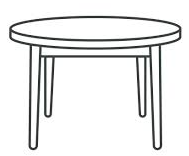
\includegraphics[scale=0.45]{../img/tavolo.png}
\end{center}

Pyhsical object with elestic characteristics can be exited in some way producing sound waves.

\begin{center}
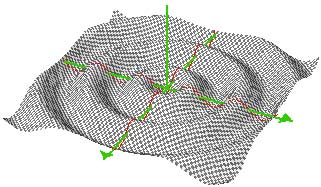
\includegraphics[scale=0.55]{../img/pelle.png}
\end{center}

Sound waves are a form of energy that propagates in time and space through an elastic medium.

Sound waves simply exist in our world.

When a sound wave reaches our ears it is perceived as an acoustic information by our brain.

\begin{center}
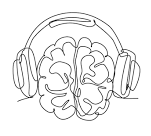
\includegraphics[scale=0.5]{../img/percezione.png}
\end{center}

It's a concrete thing.

When it was choosen or assembled:

\begin{itemize}
\tightlist
\item we can interact with it (touch it, move it, etc.).
\item we can make a copy (a model).
\item we can modify it (improve it).
\item we can destroy (or forgot) it.
\item it does not require linguistic representation, it simply be.
\item it exist in space and not necessary in time.
\end{itemize}

This has to do with the physical world.

We live immersed in sound waves.

We listen to music more or less daily but\ldots is music always sound waves?

No.

We can think and organize sounds inside our mind without producing them as sound waves.

\begin{center}

\includegraphics[scale=0.65]{../img/musicervice.png}
\end{center}

Sound waves have to do with physical world and human perception.

Music is a complex thing that has to do with both perceptual and cognitive human systems.

\subsection{Pre-linguistic}\label{pre-linguistic}

We can compose ideas or instinctive sequences of sounds.

Putting thoughts together in a pre-linguistic manner.

\begin{center}
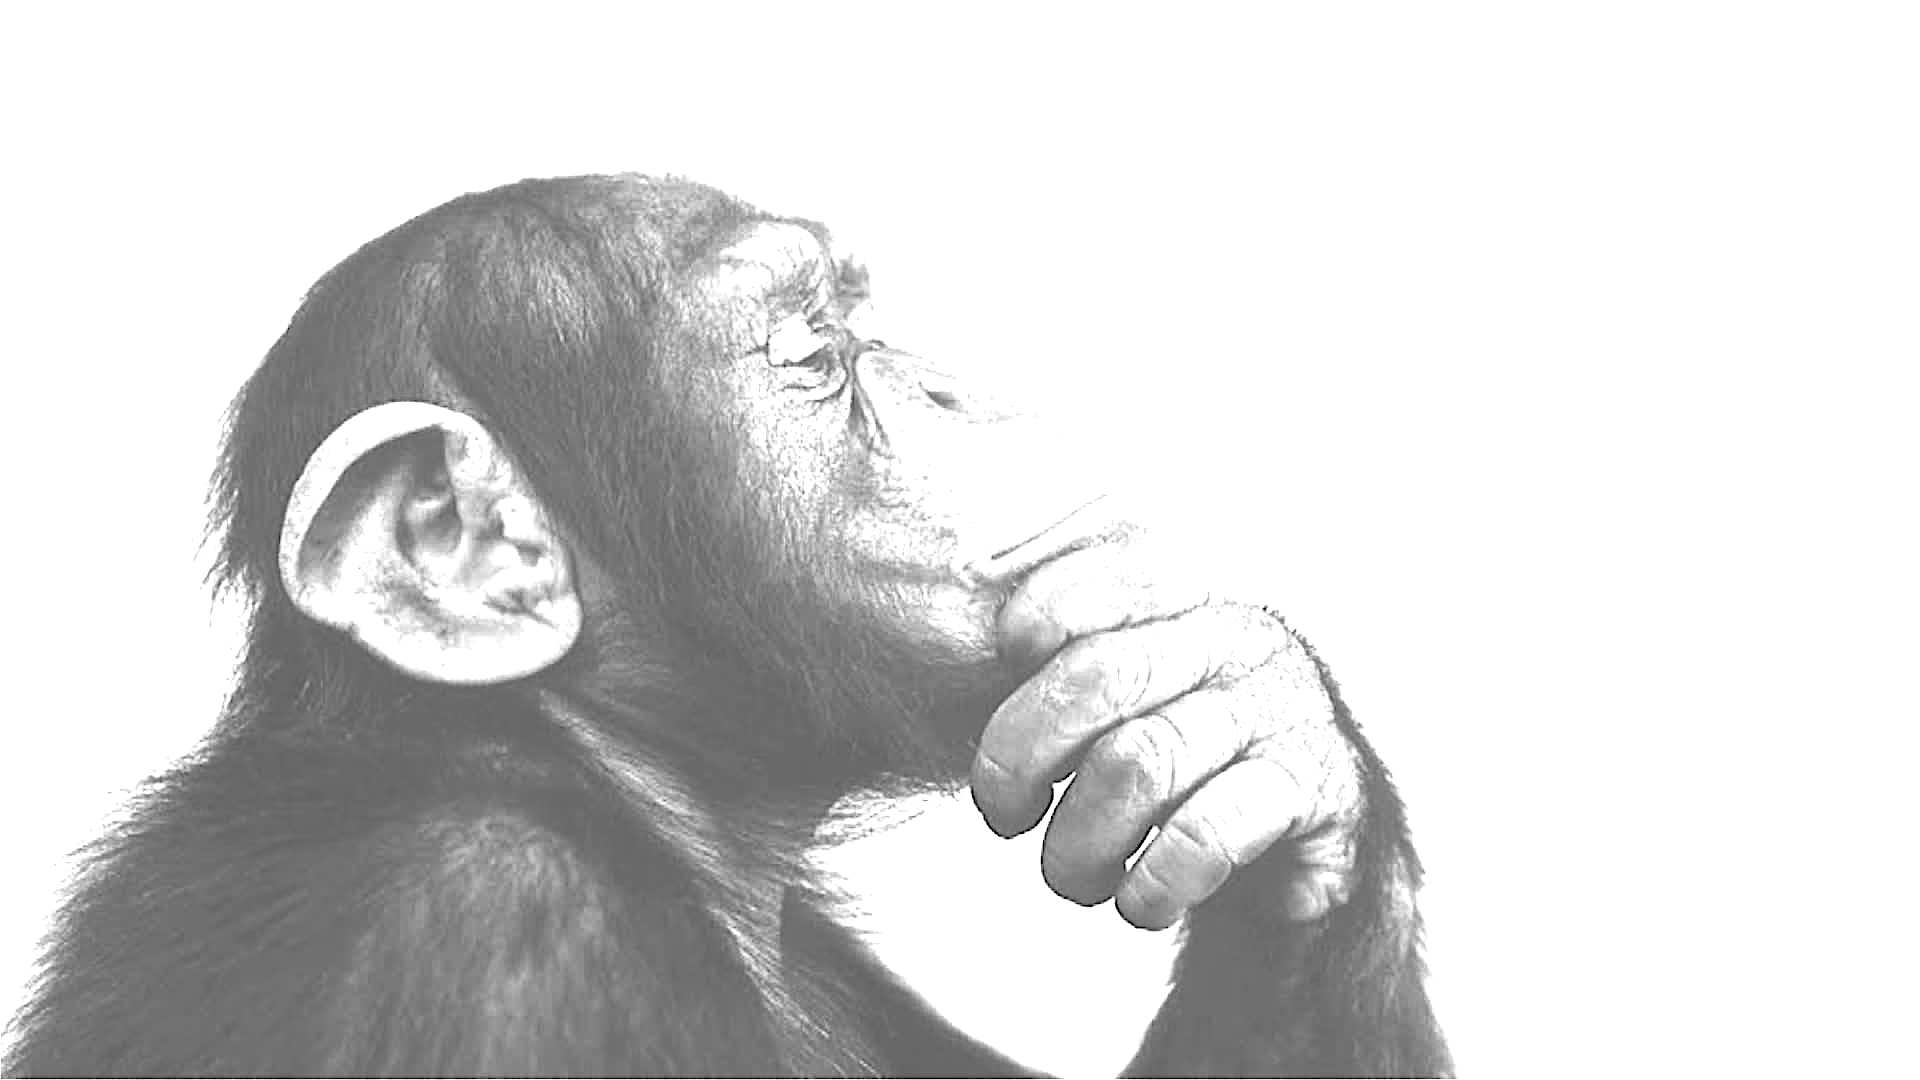
\includegraphics[scale=0.35]{../img/pensiero.png}
\end{center}

An abstract thing.

When we thinked it:

\begin{itemize}
\tightlist
\item we can't interact with it (touch it, move it, etc.).
\item we can do a copy (replicate pattern structure).
\item we can reproduce it but only in its physical forms (kinds of matter):
   \begin{itemize}
   \tightlist
   \item declaiming it (sound waves).
   \item writing it on a paper using symbolic representations.
   \end{itemize}
\item we can modify it.
\item we can't destroy it (we can only destroy its representation in physical world - book, recordings, etc. - not in our memory).
\item it does not require linguistic representation.
\item it exists in the space of consciousness (our mind) but when we
  reproduce it in the physical world it exist both in space and time.
\end{itemize}

This has to do with mind, consciousness and human expression.

Let's explore this concept through a comparison between natural language and musical language because they: 
\begin{itemize}
\tightlist
\item are universal (present in all human cultures). 
\item belong exclusively to our species. 
\item ensure the cohesion of a social group. 
\item share formal and functional characteristics.
\end{itemize}

\subsubsection{Natural language}\label{natural-language}

Psycholinguistic studies say that at a deep level all natural languages have the same structure and this can tell us something universal about the human intellect (our brain).

The form of human thought is innate and common to all members of the species.

The function of language is to express it.

\begin{center}

\includegraphics[scale=0.5]{../img/linguaggio.png}
\end{center}

The deep structure of an expression is closely related to the thought it represents.

If pre-linguistic thoughts have the same type of form for everyone the linguistic structures that represent them must also have the same type of form.

\begin{center}
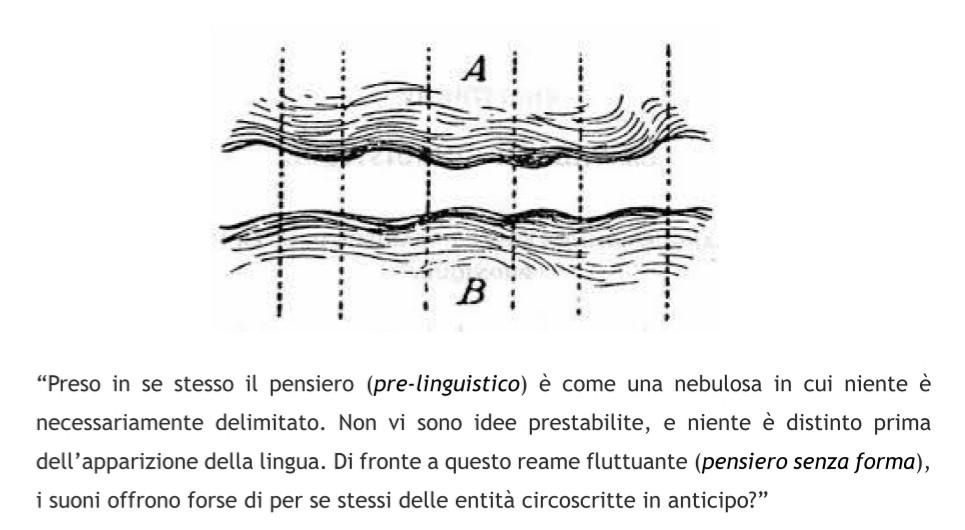
\includegraphics[scale=0.4]{../img/prelinguistico.png}
\end{center}

If we want to transform a deep thought structure into a statement we assemble it together into a linear sequence of sounds.

This sequence must convey to the listener the necessary informations for its comprehension.

Thought itself cannot be considered a linguistic sequence because it exists independently of language.

\subsubsection{Musical language}\label{musical-language}

About music there exist forms of mental activity independent of any musical language such as \href{http://www.musicaecodice.it/gitmedia/emc/1_media/bimbi.mp3}{children's nursery rhymes} or \href{http://www.musicaecodice.it/gitmedia/emc/1_media/tibet.mp3}{tibetan songs}.

Pre-linguistic musical thought must be an abstract scheme that includes exclusively the characteristics common to all musics.

If both music language and natural language are universal characteristics of the human specie this means that humans have a natural capacity to acquire both linguistic and musical skills.

Natural language and musical language expressions are conveyed in the real world in the form of sound waves.

The sound waves common basic physical parameters are: 

\begin{itemize}
\tightlist
\item frequency \(\rightarrow\) interval, pitch, intonation. 
\item amplitude \(\rightarrow\) dynamic. 
\item time \(\rightarrow\) rhythm. 
\item timbre \(\rightarrow\) instrumental techniques, vocal expressions, orchestration.
\end{itemize}

Even though surface forms differ from culture to culture we can find these universal elements not only in physical parameters but also in the subdivision into multiple levels of the languages.

\subsection{Compose a phone number}\label{compose-a-phone-number}

\begin{center}

\includegraphics[scale=0.4]{../img/telefono.png}
\end{center}

Defining a code.

\begin{itemize}
\tightlist
\item a sequence of numbers (or letters or sounds) that represents a thought.
\item we can't modify it.
\item it requires encoding and decoding.
\item to understand it we need to know its linguistic structure.
\item it follow precise and shared rules.
\item if we don't know them, the sequence of numbers or sounds makes no sense to us.
\item it require linguistic representation.
\item it can be: 
  \begin{itemize}
  \tightlist
  \item in space \(\rightarrow\) if you write it in a phone directory.
  \item in time \(\rightarrow\) if you digit it on a phone keyboard.
  \end{itemize}
\end{itemize}

This has to do with language and its representations.

Let's start again with the comparison between natural and musical language.

Leaving aside the first common level represented by the physical parameters of sound both are built on further different levels.

Simplifying, we can identify four levels:

\begin{itemize}
\tightlist
\item phonetic-phonological \(\rightarrow\) phonetics and prosody - individual notes, pitches, scales, tunings, etc.
\item morphosyntactic \(\rightarrow\) combination of phonemes into morphemes and morphemes into words - rhythm, chords, etc.
\item syntactic \(\rightarrow\) rules defining the relationships between words - counterpoint, harmony, twelve-tone system, asides, phrases, etc.
\item semantic \(\rightarrow\) access to meaning.
\end{itemize}

\subsubsection{Phonetic-phonological level }\label{phonetic-phonological-level}

It is present in all languages.

Every linguistic output can be broken down into phonemes which are a small set of sound classes.

For example the word `ape' is made up of three phonemes one for each letter.

Phonemes have two distinctive features: 

\begin{itemize}
\tightlist
\item they are not characterized by absolute values but by a set of sounds within a certain range. 
\item the continuum of sounds is divided differently in different languages (two sounds that constitute two phonemes in one language form a single phoneme in another).
\end{itemize}

\begin{center}
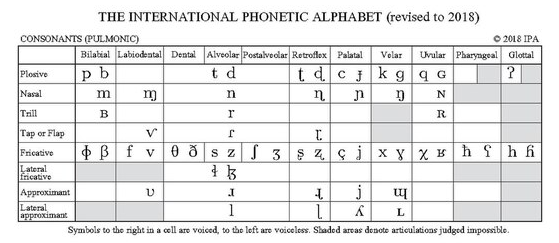
\includegraphics[scale=0.9]{../img/fonemi_2.png}
\end{center}

In western musical languages the fundamental phoneme could be considered the note with its various types of expression (staccato, tenuto, accentato, legato, etc.).

\begin{center}

\includegraphics[scale=0.22]{../img/nota.png}
\end{center}

Let us remember that in both languages they are characterised by frequency, duration, amplitude and timbre.

\subsubsection{Morphosyntactic level }\label{morphosyntactic-level}

Phonemes can join together to form morphemes.

Morphemes can join together to form words.

Words are basic elements of language that: 

\begin{itemize}
\tightlist
\item carries meaning. 
\item can be used on its own.
\item are uninterruptible.
\end{itemize}

In music we could consider them as a short melodic pattern (inciso).

\begin{center}
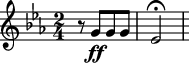
\includegraphics[scale=0.7]{../img/inci.png}
\end{center}

A vocabulary (lexicon) is a set of words in a given language.

In music we could consider it as a set of rhytmic and melodic patterns.

Substantial differences between the two languages:

\begin{itemize}
\tightlist
\item in natural language a word has a general function (the word `table' represent a table).
\item in music a specific word exist only within a piece (we can consider Beethoven's fifth symphony incise a word only in this symphony).
\end{itemize}

\subsubsection{Syntactic level }\label{syntactic-level}

Syntax or formal grammar \(\rightarrow\) a closed system of rules that serves exclusively to generate the set of sequences considered grammatical.

Every natural language like every musical language has its own syntax (Italian, French, German, counterpoint, harmony, twelve-tone, etc.).

We have previously defined that music is not necessarily conveyed through sound waves but\ldots are sound waves always music?

No, again.

In order to be defined music language requires a codification of sounds in vocabularies and systems of rules.

\begin{center}
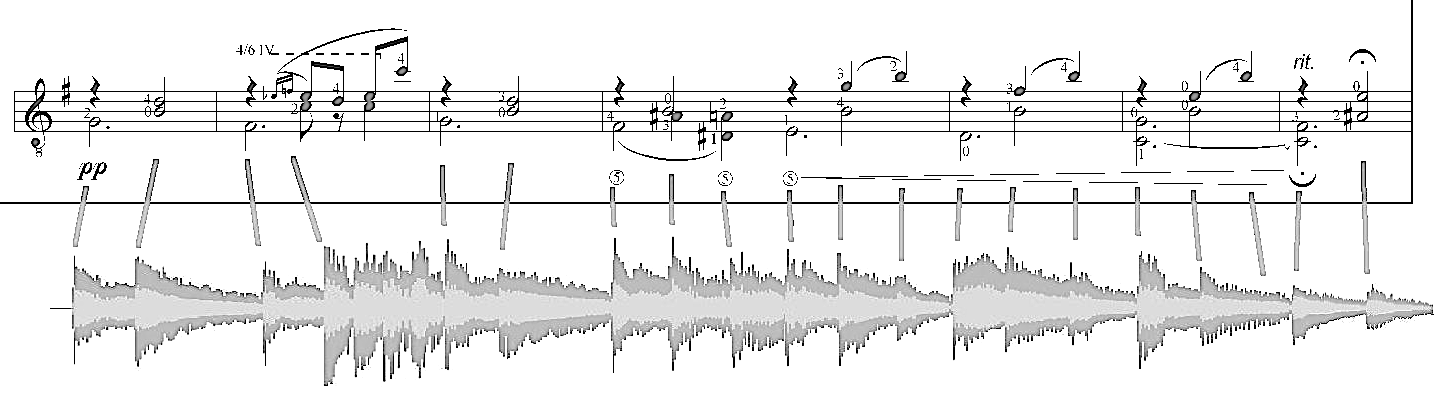
\includegraphics[scale=0.9]{../img/ondenote.png}
\end{center}

In all musical cultures the physical parameters of sound are organized in symbols.

These symbols can become independent from sound waves.

\begin{center}
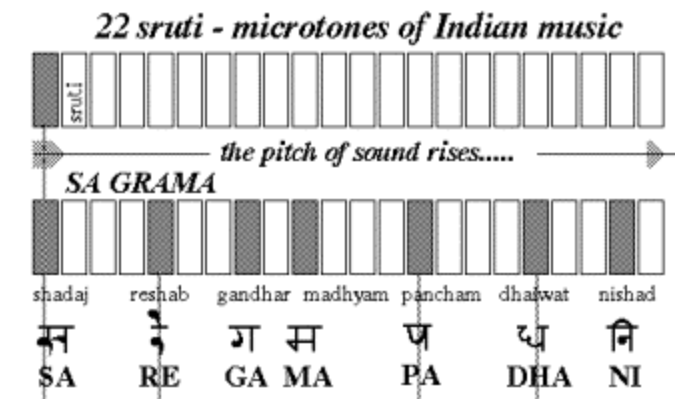
\includegraphics[scale=0.4]{../img/india.png}\break
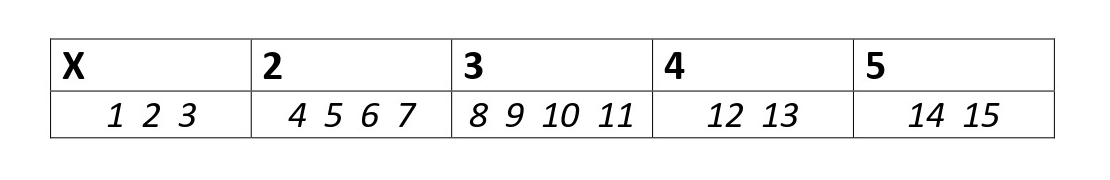
\includegraphics[scale=0.3]{../img/rtmoindia.png}
\end{center}

In Western musical tradition, from psamody until around 1940 these parameters have maintained more or less the same vocabulary over the centuries (diatonic and chromatic intervals, metric and subdivision of beat, musical instruments, etc.).

\begin{center}
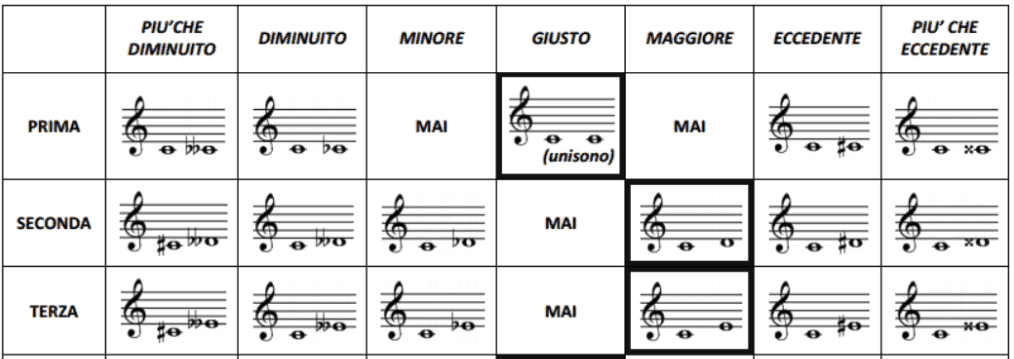
\includegraphics[scale=0.85]{../img/intervalli.png}
\end{center}

The systems of rules through which the vocabulary terms were organized (syntax), however, were different (modality, counterpoint, harmonic systems, dodecaphony, stocastic systems, alea, etc.).

\begin{center}
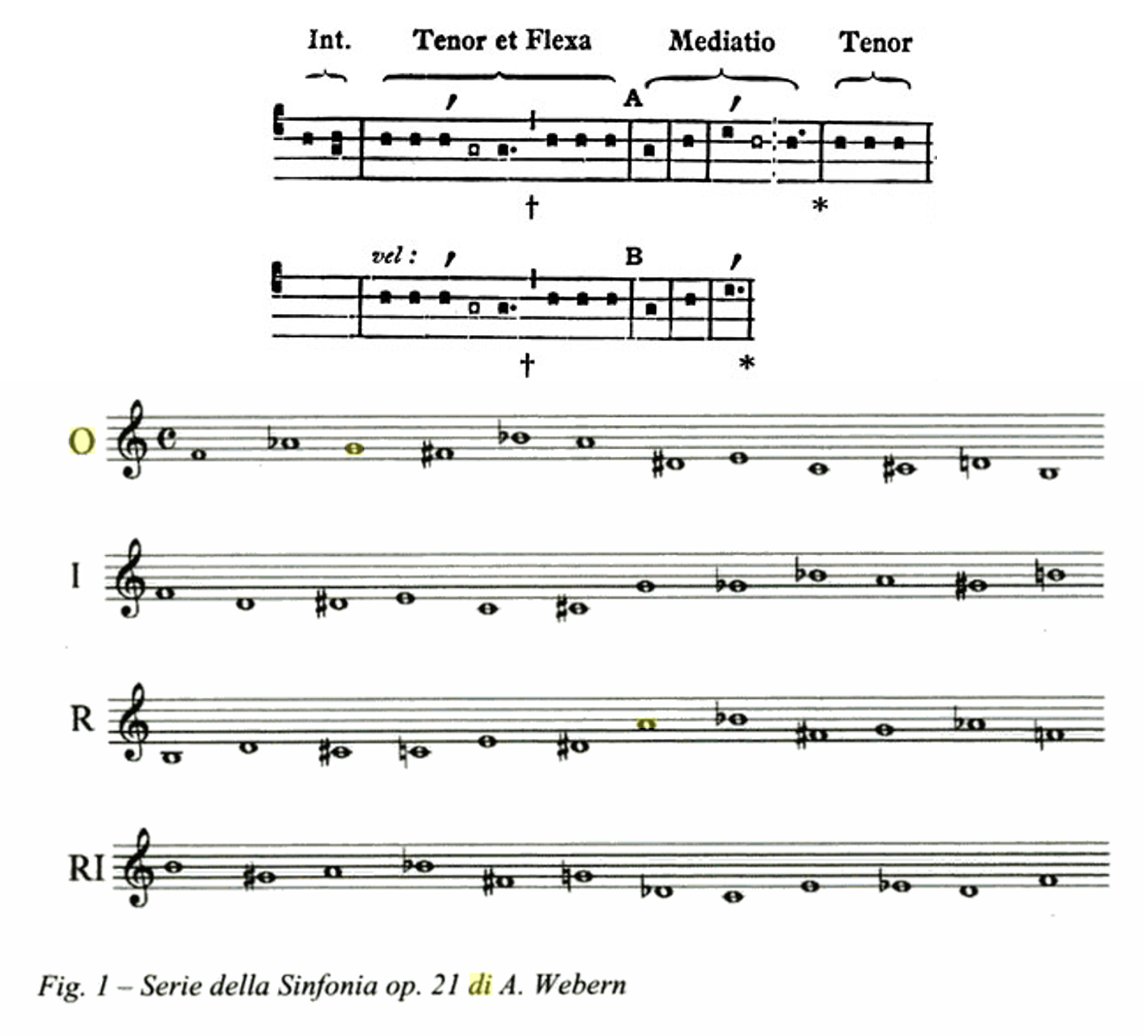
\includegraphics[scale=0.75]{../img/greg.png}
\end{center}

For this reason we cannot define western music as a single language but as a set of languages \hspace{0pt}\hspace{0pt}that use the same vocabulary (classical music, baroque music, pop music, jazz music, etc.).

Even more so if we talk about music from different cultures.

On this level the differences underlined at the end of the previous paragraph regarding musical words disappear.

Musical grammars are a meta-reflection that deals with symbolic forms.

These can be abstracted to the point of taking on a meaning of their own that goes beyond the perception of the work.

\begin{center}
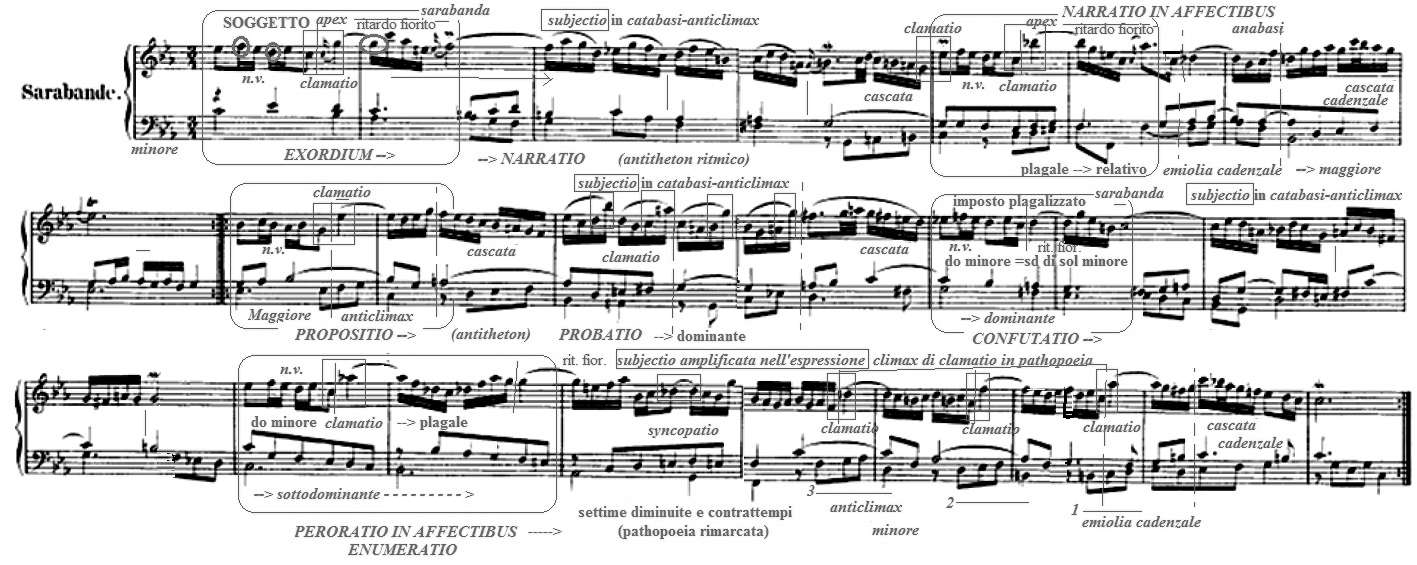
\includegraphics[scale=1.1]{../img/analisische.png}
\end{center}

\subsubsection{Semantic level}\label{semantic-level}

The branch of linguistics and logic concerned with meaning.

In musical language there are several starkly contrasting theories on this subject none of which can be assumed to be universal.

The one that summarizes the two main positions was proposed by the American musicologist L.B.Meyer who distinguishes between two forms of meaning in music:

\begin{itemize}
\tightlist
\item designative meaning \(\rightarrow\) which refers to something extramusical (G.Malher \href{http://www.musicaecodice.it/gitmedia/emc/1_media/malher.mp3}{Symphony n 10} - extract).
\item embodied meaning \(\rightarrow\) the meaning a piece has for the listener in terms of:

  \begin{itemize}
  \tightlist
  \item Internal syntactic structure.
  \item Interactions between this structure and the listener's musical knowledge and expectations. Musical structure can create expectations that can be disappointed or fulfilled generating a dynamic flow of tensions and resolutions that influence the listener's emotional and aesthetic responses. These are aesthetic emotions that have nothing to do with the emotions experienced in real life (F.Schubert \href{http://www.musicaecodice.it/gitmedia/emc/1_media/schubert.mp3}{Trio} - extract).
  \end{itemize}
\end{itemize}

Can we express in words what emotions listening to this Schubert trio arouses in us?

We will delve deeper into this last topic in the \hyperref[meaning]{Music’s meaning} section.

These levels enable common phenomena that help us understand the difference between sound waves and language.

\begin{itemize}
\tightlist
\item categorical perception \(\rightarrow\) a continuous linguistic or musical sound is segmented into discrete categorized units (phonemes, notes, words). If we repeat the same phrase or melody several times they will always be recognized as the same despite variations in acoustic parameters sometimes even significant ones (\href{http://www.musicaecodice.it/gitmedia/emc/1_media/pollini.mp3}{exemple 1}, \href{http://www.musicaecodice.it/gitmedia/emc/1_media/kissin.mp3}{exemple 2}, \href{http://www.musicaecodice.it/gitmedia/emc/1_media/sokolov.mp3}{exemple 3}).
\item phonemic restoration \(\rightarrow\) replacing part of the linguistic signal with noise simultaneously with the word or music does not affect the perception of the whole. Semantic-lexical or musical expectations prevail over acoustic analysis (\href{http://www.musicaecodice.it/gitmedia/emc/1_media/buchi.mp3}{musical},  \href{http://www.musicaecodice.it/gitmedia/emc/1_media/vian.mp3}{natural}).
\item expectations \(\rightarrow\) the syntactic construction of a sentence leads us to expect one word rather than another within it, just as happens within a sequence of chords in tonal terms (\href{http://www.musicaecodice.it/gitmedia/emc/1_media/analisi.mp3}{words}, \href{http://www.musicaecodice.it/gitmedia/emc/1_media/accordi.mp3}{chords}).
\end{itemize}

\subsection{Perceive and process }\label{perceive-and-process}

The ability to perceive and process musical information (not exclusively acoustic) is also common to all cultures.

Listening to music from one's own culture provides the listener with additional implicit information.

The simplest musical competence requires the activation of numerous cognitive abilities, including: 

\begin{itemize}
\tightlist
\item memory \(\rightarrow\) short-term recognition of melodic rhythmic patterns.
\item maintenance of attention \(\rightarrow\) active listening.
\item analysis of the temporal structure \(\rightarrow\) continuous comparison between present and short-term memory.
\end{itemize}

These abilities are part of a body of knowledge acquired through more or less conscious implicit learning that occurs through two modalities:

\begin{itemize}
\tightlist
\item universal cognitive mechanisms \(\rightarrow\) experimental psychology studies have shown that even prenatally the fetus responds to sounds and noises that activate phonological priming processes. For example, infants have been found to prefer sounds or stories frequently reproduced by their mothers after the third month of pregnancy over
those they have never heard. Even in adulthood, some research has highlighted the existence of perceptual mechanisms independent of cultural context.

\item environmental and cultural interaction \(\rightarrow\) constant, quantitatively preponderant, continuous and more or less conscious perception of sounds organized according to the reference syntax of the cultural environment of reference.
  
\begin{center}
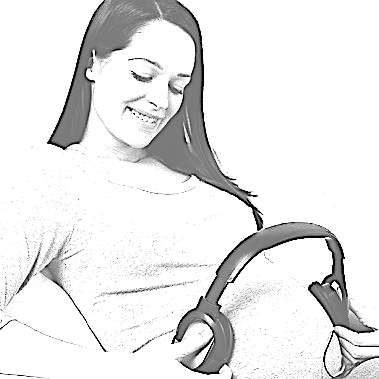
\includegraphics[scale=0.28]{../img/prenatale.png}

\includegraphics[scale=0.55]{../img/metro.png}
\end{center}
\end{itemize}

An example of the dichotomy just described can be found in analyzing the pitches of a melody.

To accomplish this we must activate several cognitive mechanisms which, in their simplest form are:

\begin{itemize}
\tightlist
\item processing the melodic profile (the progression of the ups and downs)  \(\rightarrow\) occurs more easily in both children and adults, with or without musical experience or literacy.
\item processing musical intervals (the distance between pitches) \(\rightarrow\) occurs less easily in general and to a greater extent in individuals with more experience or musical literacy (\href{http://www.musicaecodice.it/gitmedia/emc/1_media/veloso.mp3}{melody}).
\end{itemize}

\subsection{Re-compose a puzzle}\label{re-compose-a-puzzle}

\begin{center}
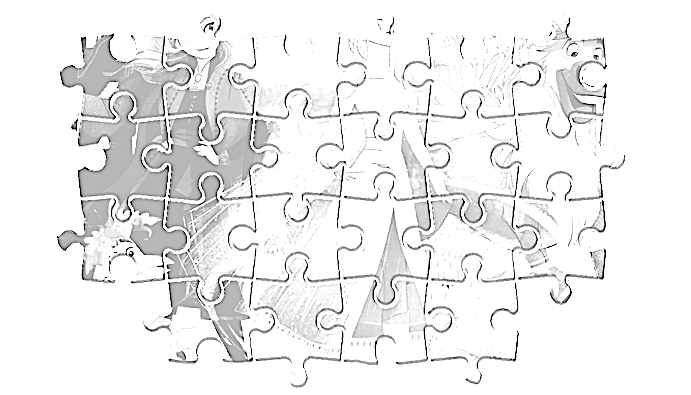
\includegraphics[scale=0.3]{../img/puzzle.png}
\end{center}

Re-constructing an image.

An abstract thing reconstructed in the physical world through a sequence of actions.

\begin{itemize}
\tightlist
\item we continuously interact between abstract and real world through attempts to correctly reproduce the original image.
\item we can reproduce the process many times but we cannot consider them copies.
\item we can't modify it.
\item it does not require necessary linguistic representation but cognitive skills.
\item during the re-composition process it need time and space but when the process is ended it need only space (in the case of a musical reproduction a space in our memory and consciousness).
\end{itemize}

This has to do with music representations, interpreters, players and performers.

Up to now we have thought about sound, music and their perception but not about the actors involved in the process of making music.

\begin{itemize}
\tightlist
\item composer.
\item interpreter.
\item listener.
\end{itemize}

We will delve deeper into these concepts in a dedicated paragraph \textit{Forms of human expression}.

\section{Music's meanings }\label{musics-meanings}

When we talked about the semantic level we mentioned the meaning but\ldots what is the meaning of music and what does music represent for humans?

We start again with sound waves \(\rightarrow\) it represent music in the physical world like clouds or mountains.

This has to do with both perceptual and cognitive processes.

By abstraction we can consider sound waves as \href{http://www.musicaecodice.it/gitmedia/emc/1_media/segno1.mp4}{signs}.

Let's think on these topics: 

\begin{itemize}
\tightlist
\item their production, transmission and interpretation. 
\item the ways in which something is communicated and signified. 
\item the production of symbolic objects.
\end{itemize}

\subsection{Signs and sounds }\label{signs-and-sounds}

\begin{center}

\includegraphics[scale=0.45]{../img/montagne.png}
\end{center}

\begin{itemize}
\tightlist
\item let's go hiking
\item we're driving on a mountain road.
\item we see cars parked on the side of the road.
\item we realize that the mountain path we're looking for probably starts there.
\end{itemize}

We can consider the many parked cars a sign that indicated the beginning of the trail.

Our intentions, the context, and the tracks we encountered along the way activated within us an action-reaction mechanism made up of perceptions, expectations, emotions, interpretations, etc.

We can define:

\begin{itemize}
\tightlist
\item the sight of the group of cars \(\rightarrow\) the signifier (plane of expression) --- what made us understand something.
\item the presence of the beginning of the trail \(\rightarrow\) the signified (plane of content) --- what we understood.
\end{itemize}

Speaking semiotically the union of these two elements gives rise to a sign that generates an increase in knowledge.

Having found the beginning of the trail is what we can call the paradigmatic effect of the sign (we were looking for something and we found it).

Listen (\href{http://www.musicaecodice.it/gitmedia/emc/1_media/uccellini.mp3}{exemple 1}, \href{http://www.musicaecodice.it/gitmedia/emc/1_media/bach_1.mp3}{exemple 2}, \href{http://www.musicaecodice.it/gitmedia/emc/1_media/berio.mp3}{exemple 3}) and answer.

\begin{enumerate}
\def\labelenumi{\arabic{enumi}.}
\tightlist
\item what kind of information do they provide us?
\item what is the signified content of these acoustic expressions?
\item what kind of increase in knowledge was achieved after listening to them?
\end{enumerate}

These short sound texts could refer to three classic genres of electroacoustic music: soundscape composition, computer music and tape music.

All are carried by sound waves but have profoundly different signified contents that cannot be deduced (or composed) starting from the acoustic parameters of the sound.

\subsection{Composers, players and listeners }\label{composers-players-and-listeners}

\begin{center}

\includegraphics[scale=0.6]{../img/nuvole.png}
\end{center}

Come back to the mountain path.

\begin{itemize}
\tightlist
\item we're walking on the path.
\item the clouds are gathering \(\rightarrow\) signifier.
\item we understand that it's about to rain \(\rightarrow\) signified.
\item we decide to come back to the car \(\rightarrow\) practical effect.
\end{itemize}

Signs often have a practical effect.

Sounds often have a practical effect (hearing thunder is like seeing clouds).

Have music pratical effect?

Signs connect: 
\begin{itemize}
\tightlist
\item something perceptual \(\rightarrow\) the sight of cars or clouds with 
\item something cognitive \(\rightarrow\) the presence of the path or impending rain.
\end{itemize}

Signs are not signifiers \(\rightarrow\) their perception by someone is.

A sign is not something that represents something else.

It represent the relationship someone establishes between two elements:

\begin{itemize}
\tightlist
\item a perceptible dimension (the view of the clouds). 
\item  an intelligible dimension (we connect it to the possibility of rain).
\end{itemize}

This relationship: 

\begin{itemize}
\tightlist
\item occurs \textit{a posteriori}.
\item is not necessarily intentional on the part of the sender (clouds are not harbingers of rain, just as the person who parked on the side of the road didn't mean to tell us the start of the trail).
\end{itemize}
We can connect signifier and signified only through an experiential factor (previously, when we saw those clouds, it rained).

\begin{center}
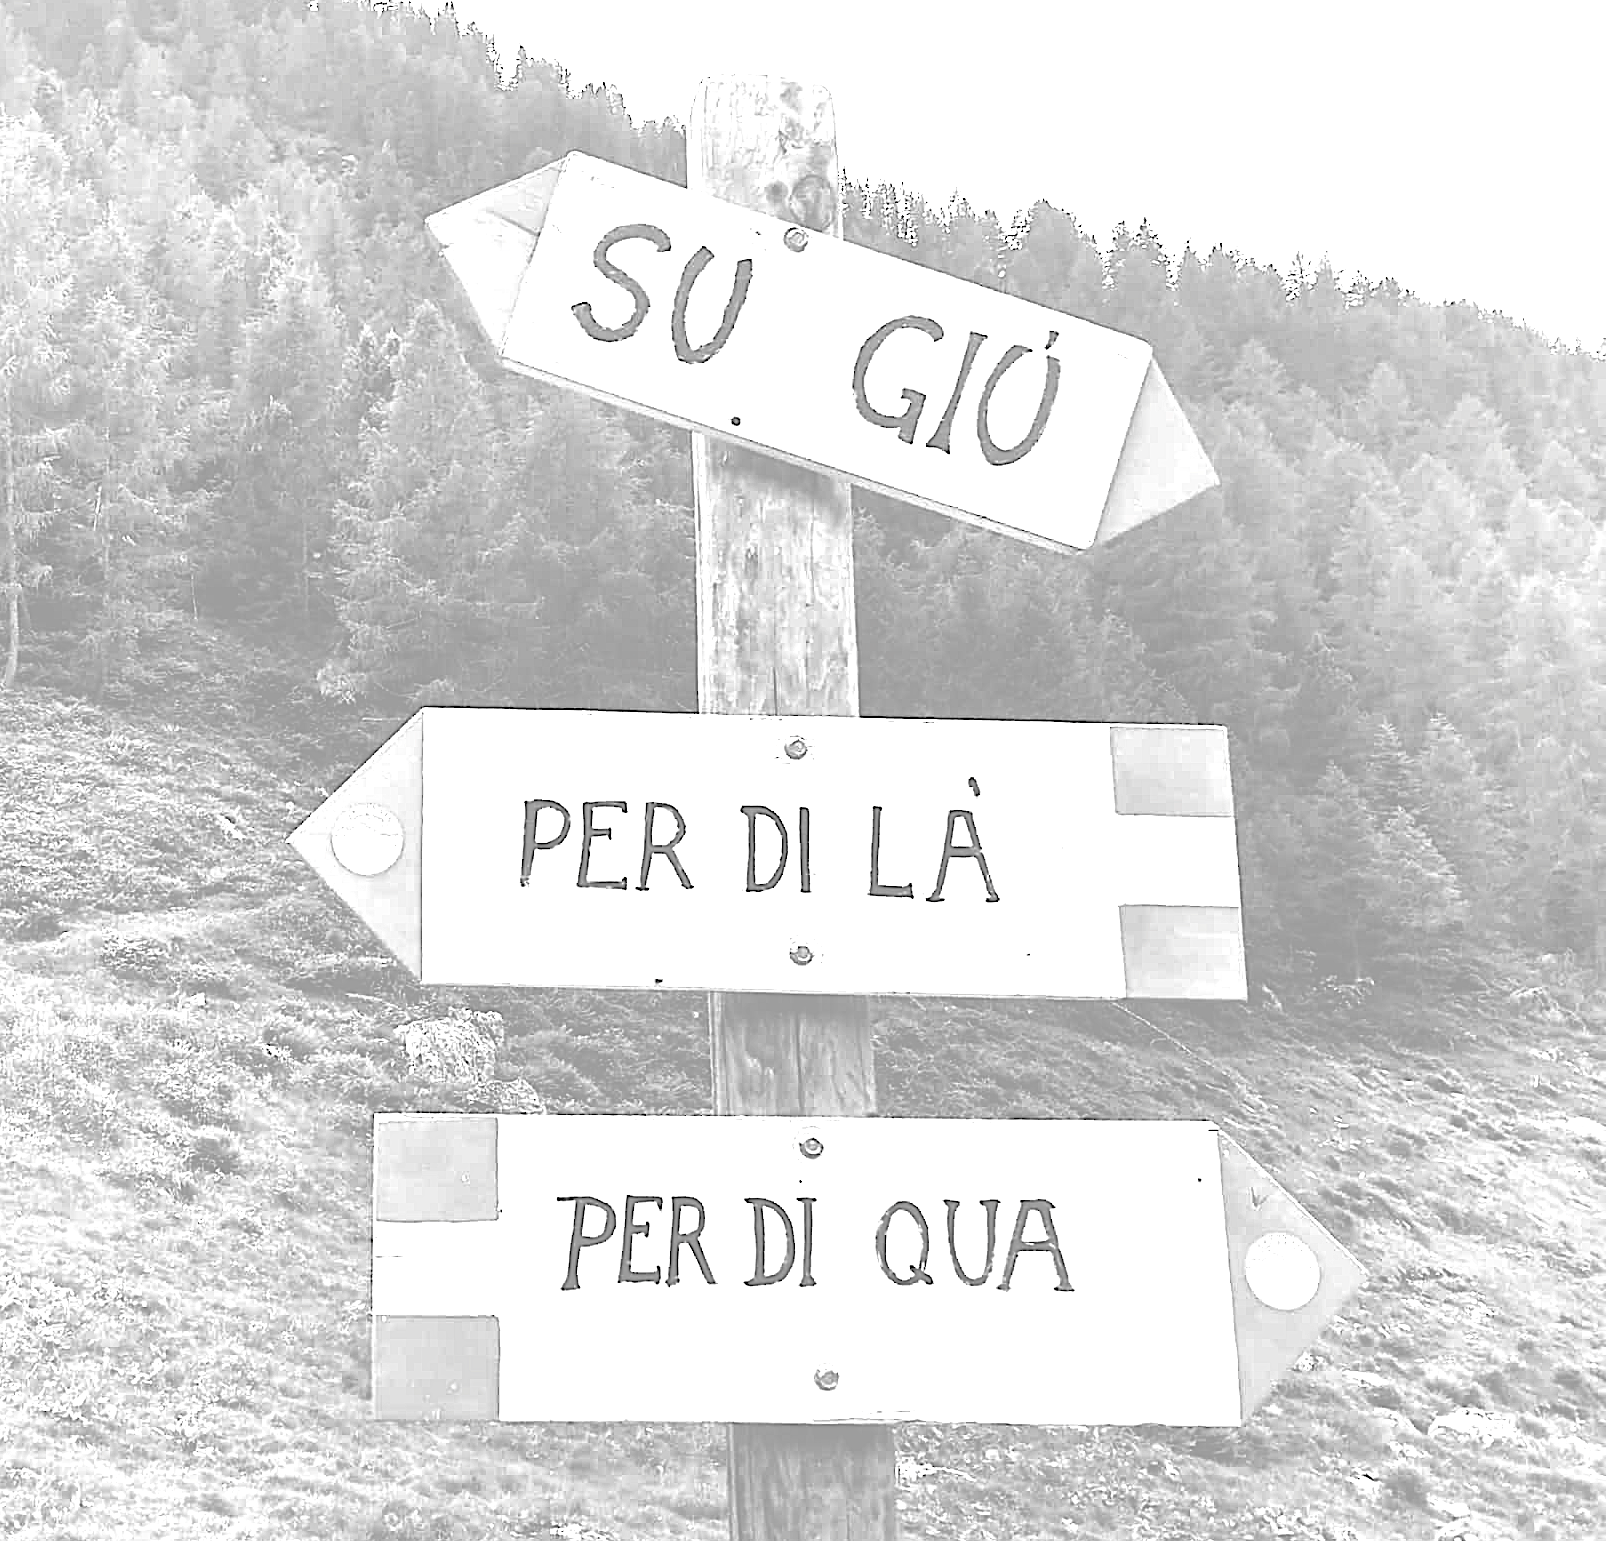
\includegraphics[scale=0.4]{../img/cartello.png}
\end{center}

Signification \(\rightarrow\) as the examples just given, we are constantly surrounded by a multiplicity of unconsciously produced signs.

All these signs have the potential to become signifier expressions if interpreted by a recipient in the general act we can define as signification.

Communication \(\rightarrow\) the sign is voluntarily produced by the emitter to convey a message, such as the signs in the previous image or the same images within this text.

Listen (\href{http://www.musicaecodice.it/gitmedia/emc/1_media/annuncio.mp3}{exemple 1}, \href{http://www.musicaecodice.it/gitmedia/emc/1_media/pubbli.mp3}{exemple 2}, \href{http://www.musicaecodice.it/gitmedia/emc/1_media/ligeti.mp3}{exemple 3}) and answer.

\begin{itemize}
\tightlist
\item what is the practical effect of the three sound texts?
\item is sound information contained in the acoustic properties of the sound texts?
\end{itemize}

Sounds can be both signification and communication.

Music can be only comunication.

In the performing arts of non-oral traditions (such as the western musical tradition), things get even more complicated because several actors play in the communication process:

\begin{itemize}
\tightlist
\item composer \(\rightarrow\) usually thinks of a composition in his mind (symbolic musical language) and then represent it through some kind of notational code on a score.
\item score \(\rightarrow\) the coded instructions needed by an interpreter to reproduce the composer's ideas in the physical world in the form of sound waves.
\item interpreter \(\rightarrow\) must know both the musical language used by the composer and the symbolic language through which it was codified (semiography).
\item listener \(\rightarrow\) receiver that interprets an interpretation.
\end{itemize}

In acoustic music it is always like this, while in electroacoustic music things can change.

\subsection{Do you know this music? }\label{do-you-know-this-music}

\begin{center}
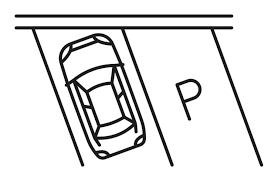
\includegraphics[scale=0.4]{../img/parcheggio.png}
\end{center}

What is the relationship between signifiers and signifieds activated bythe receiver based  on?

Is this relationship always valid and somehow implicit in the signifier, or does it depend on context and conditions?

Let's consider the example of clouds and rain.

There is no an universal law that says that every time there are clouds in the sky, it will rain.

The relationship is established through `a posteriori' inductive generalization codified in an interpretative rule \(\rightarrow\) it often rained after observing clouds in the sky, and therefore, whenever we encounter clouds, we associate them with the phenomenon.

Does this also apply to the example of cars parked on the side of the road?

In this case:

\begin{itemize}
\tightlist
\item there isn't an universal law according to which every time we observe parked cars, a mountain path is nearby.
\item there isn't an interpretative rule established by inductive generalization, since parked cars rarely indicate the start of a trail.
\end{itemize}

The way of reasoning that led to the signification (inference) was induced:

\begin{itemize}
\tightlist
\item by the contingent dimension \(\rightarrow\) place and context.
\item by the affective dimension \(\rightarrow\) enthusiasm for the hike, desire to find the trail to start walking, etc.
\item by the reference culture, or that set of knowledge, value systems, habits, and behaviors within which we live and which have almost naturally led us to that conclusion and not another.
\end{itemize}

The cognitive inferences used daily in our interpretations are not entirely personal or subjective \(\rightarrow\) are based on precise codes.

These codes:

\begin{itemize}
\tightlist
\item are formal systems that transcend individual choices, often imposing the use of certain mental categories.
\item are not universal.
\item are more or less lasting stabilizations of collective ways of thinking, acting, desiring, and preferring.
\item are dictated, maintained, and modified by social pressure.
\item are social and cultural customs, interpretative habits that take on the appearance of a law (without actually being one).
\end{itemize}

If we hadn't shared the same culture and been part of the same society with the many people who parked their cars on the day of the excursion, that sign simply wouldn't exist.

The sign isn't in things or ideas, but in the forms of their relationship.

Listen (\href{http://www.musicaecodice.it/gitmedia/emc/1_media/miles.mp3}{exemple 1}, \href{http://www.musicaecodice.it/gitmedia/emc/1_media/rameau.mp3}{exemple 2}, \href{http://www.musicaecodice.it/gitmedia/emc/1_media/gamelan.mp3}{exemple 3}) and answer.

Describe the differences between the three sound texts: 

\begin{itemize}
\tightlist
\item what is the first information that comes to mind when you listen? 
\item what kind of information is? 
\item are there differences between the linguistic systems used in the three sound texts? \item if there are any, what information do they influence?
\end{itemize}

Some of these arguments lead us to understand sound signs as a cultural phenomenon and not merely acoustic since from this point of view the signifier coincides with the signified.

\subsection{Do you like this music?}\label{do-you-like-this-music}

\begin{center}

\includegraphics[scale=0.4]{../img/valore.png}
\end{center}

The above codes are anthropological conventions.

The relationships between expressions and content are connected to values, preferences, and tastes, all of which are extremely complex and are:

\begin{itemize}
\tightlist
\item arbitrary \(\rightarrow\) when viewed from the outside.
\item undisputed \(\rightarrow\) when viewed from the inside.
\end{itemize}

A sign arises through difference when a sensorial discontinuity materializes, such as when, while driving along a mountain road, we encounter parked cars.

The perceptual gap brings to the surface something significant, important, which we value by distinguishing it from other signs encountered along the way.

We value it in two ways:

\begin{itemize}
\tightlist
\item we are happy because we have found what we were looking for, namely, the opportunity to embark on a beautiful hike in the mountains.
\item we have achieved what we were seeking through a journey of knowledge that has kept our attention high (observing signs, the environment, other signs, etc.) and evaluating by comparing things (would it be better to stop at a restaurant or go for an hike?).
\end{itemize}

Social codes do not completely transcend individual choices but are linked to the ways in which the individual assumes them by mediating between collective and individual values.

In summary:

\begin{itemize}
\tightlist
\item value is what we aim for and what directs our series of actions and passions, giving precise meaning to each of them according to an implicit path.
\item value arises from the evaluative comparison of things, objects, and from the recognition of differences; the greater the evaluative comparisons along the path, the greater the value.
\item the continuous mediation between collective and individual values \hspace{0pt}\hspace{0pt}generates changes in anthropological codes.
\end{itemize}

Let's see a \href{http://www.musicaecodice.it/gitmedia/emc/1_media/sordi1.mp4}{video}.

\subsection{Texts and narratives}\label{texts-and-narratives}

\begin{center}
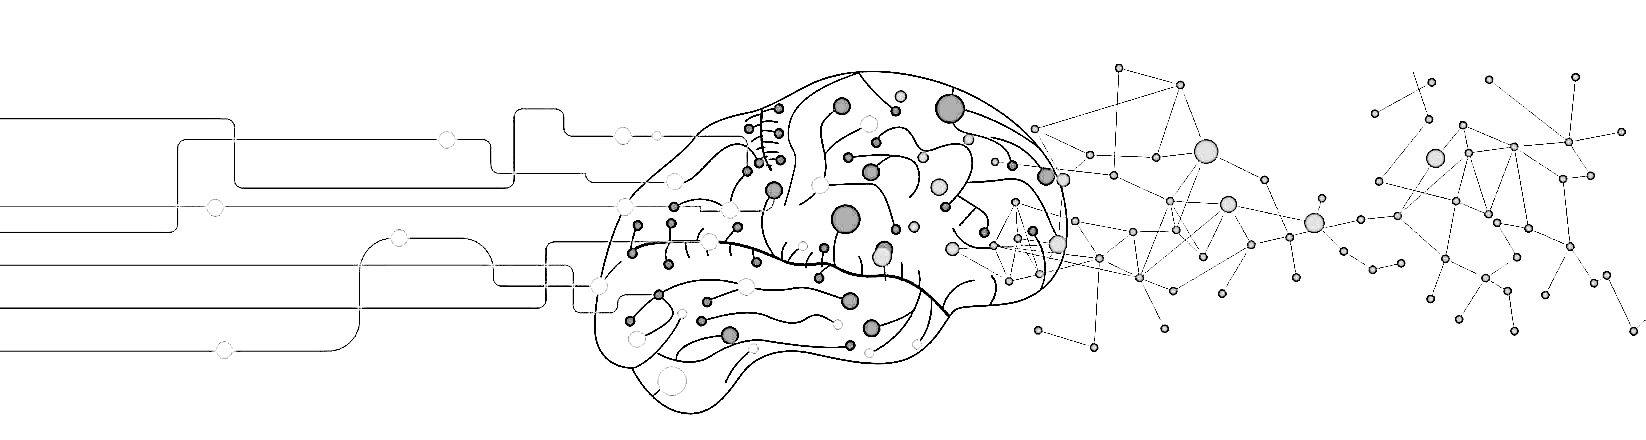
\includegraphics[scale=0.75]{../img/neuro.png}
\end{center}

The sign is just an iceberg tip.

It works because:

\begin{itemize}
\tightlist
\item it breaks down into many small, interrelated elements.
\item it composes larger entities by relating to other similar signs.
\end{itemize}

The parked cars signify the discovery of the path because:

\begin{itemize}
\tightlist
\item their unusual number in that place.
\item the way they are parked on the edge.
\item they thicken as they approach the path and then thin out.
\item they are in that place and not somewhere else.
\item they take on value thanks to differential relationships with other signs.
\item we are looking for the beginning of the path and not something else.
\item all these and other elements are part of a story that unfolds in a precise period of time.
\item this narrative is seen through a specific value-based, cultural, and anthropological perspective (a mountain hike).
\item we are in a specific emotional state (positive tension generated by the anticipation of being able to begin something we enjoy).
\item
  \ldots{}
\end{itemize}

The relationships established between these elements in a narrative generate the code through which that signifier refers to that probable meaning and not to another, forming what we might call a dynamic text.

Signs function because they are intertwined in texts.

The words of a language are like signs:

\begin{itemize}
\tightlist
\item the variable result of constant relationships between smaller elements (morphemes, phonemes, sound features),
\item themselves entities that compose larger structures (sentences, texts, speeches).
\end{itemize}

Every larger element capable of meaning transcends the smaller elements.

The meaning of a sentence transcends the meaning of the individual words that compose it, as well as the individual phonemes.

Texts are not just books, documents, etc., but any portion of the world with:

\begin{itemize}
\tightlist
\item determined limits (context).
\item precise internal articulation (code).
\end{itemize}

that carries some configuration of meaning, or better yet, a signification.

Do you remember the puzzle?

In order for meaning to:

\begin{itemize}
\tightlist
\item be produced.
\item be circulated.
\item be received.
\item be transformed.
\end{itemize}

it must refer to texts or units of meaning that various societies, historical periods, and cultures use to define their core values.

Let's see a \href{http://www.musicaecodice.it/gitmedia/emc/1_media/storia1.mp4}{video}.

\section{Forms of human expression}\label{forms-of-human-expression}

We can summarize the concepts just presented by following the thoughts of the musicologist J.J.Nattiez set out in his text `Music and discourse'.

Forms of human expression (including music) can be defined as symbolic forms only if we recognize three levels:

\begin{itemize}
\tightlist
\item poietic dimension (emitter) \(\rightarrow\) the set of strategies activated by the author that lead to the creation of the work (something that did not exist before).
\item aesthesic dimension (receiver) \(\rightarrow\) the set of strategies activated by the listener during the perception of the work.
\item the work itself (neutral) \(\rightarrow\) the text with its own internal organization that can be analyzed independently from the poietic and aesthesic dimensions.
\end{itemize}

\begin{center}
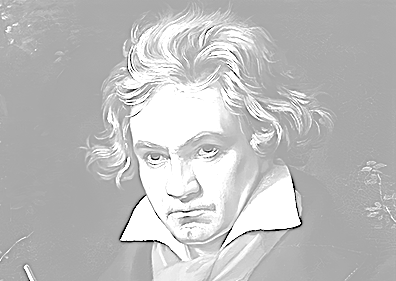
\includegraphics[scale=0.45]{../img/beethoven.png}
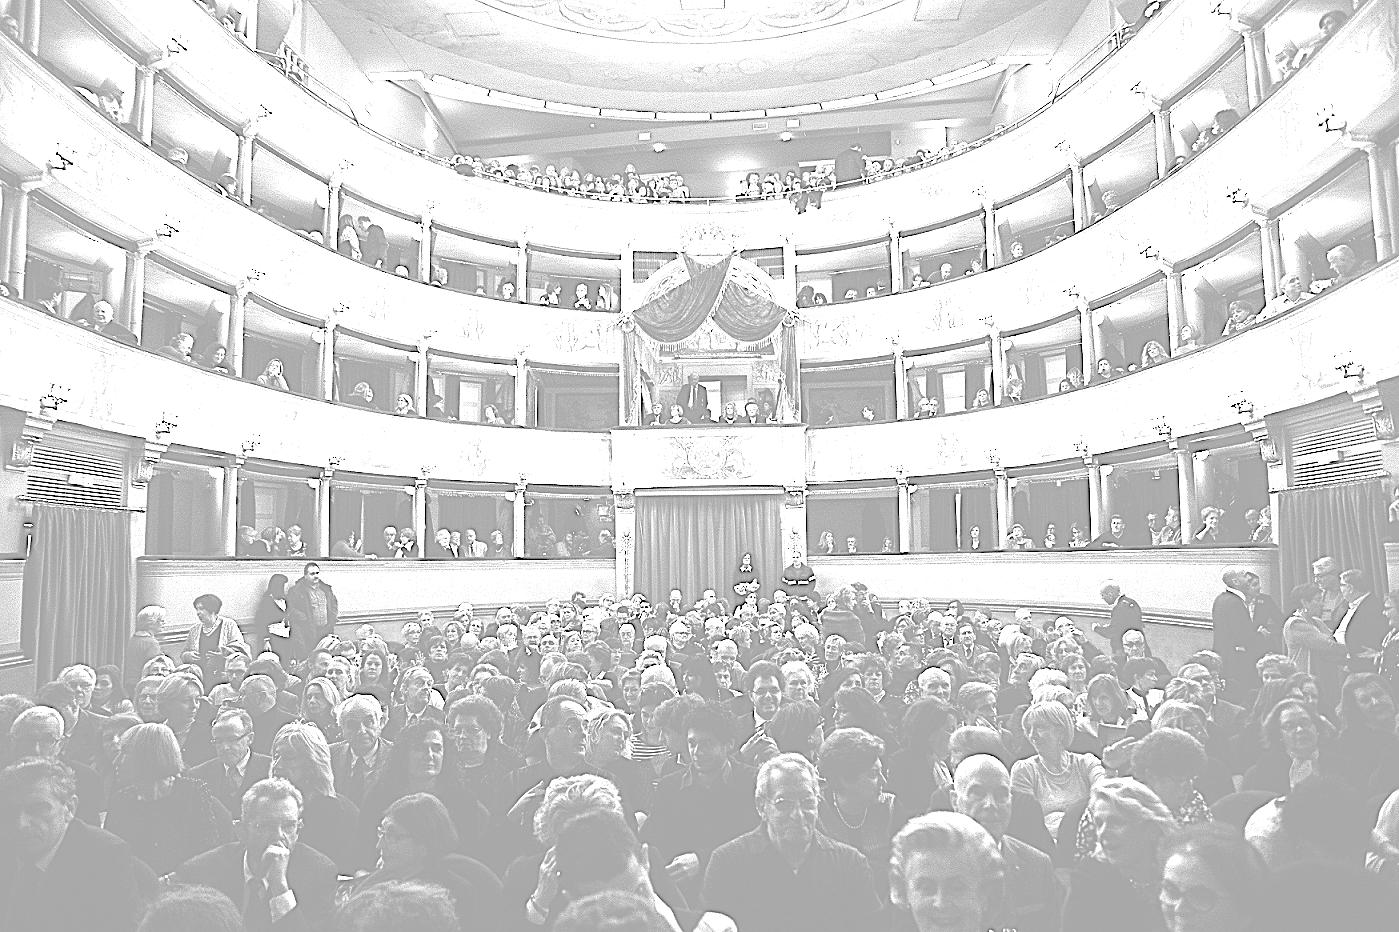
\includegraphics[scale=0.4]{../img/pubblico.png}

\includegraphics[scale=0.4]{../img/score.png}
\end{center}

\subsection{Poietic dimension}\label{poietic-dimension}

Active process of construction by the emitter (composer) of interpretant signs.

Each sign does not refer directly to an object but makes use of the intermediary action of a second sign which is its interpretant in a process of multiple references.

\begin{center}
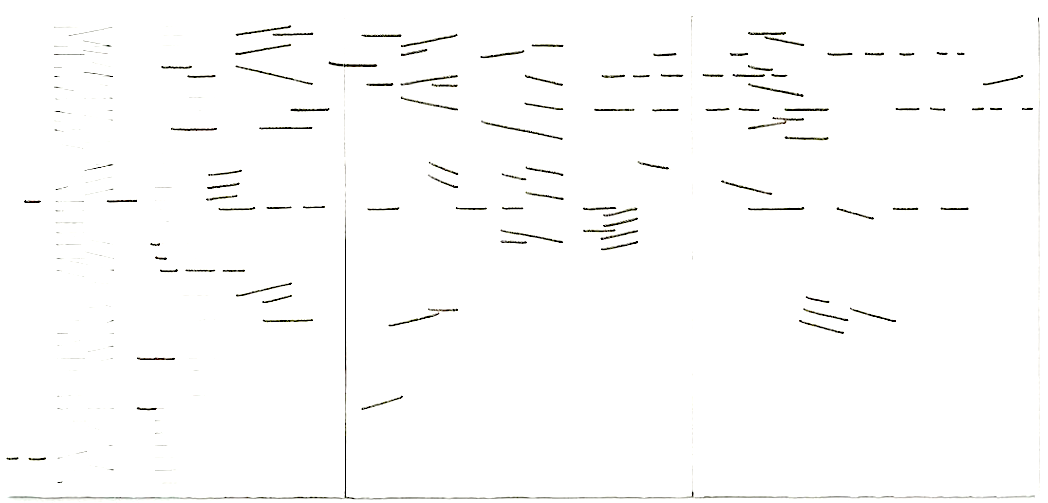
\includegraphics[scale=0.45]{../img/rimandi.png}
\end{center}

For example, in verbal language, if we write a word like table, we have:

\begin{itemize}
\tightlist
\item created a graphic sign (grapheme - formed by a sequence of letters and defined by its own rules) that, if
\item correctly interpreted by the reader, will cause him or her to pronounce the corresponding word (morpheme - sequence of phonemes defined by its own rules). If
\item correctly interpreted by the hearer, it will refer to a general idea of a table (an abstract concept defined by conventions derived from collective experience). If
\item correctly interpreted by someone, it will connect it to a real, meaningful table (object - defined by subjective experience).
\end{itemize}

This is true for a single word.

The interpretative signs become infinite when individual words are organized into a language.

Ognuno sta solo sul cuor della terra trafitto da un raggio di sole: ed è subito sera

Let's try to imagine the same process in music and the amount of control the composer can have over the \href{http://www.musicaecodice.it/gitmedia/emc/1_media/goldberg.mp3}{sound information} he wants to transmit.

\subsection{Aesthesic dimension}\label{aesthesic-dimension}

Active process of construction by the interpretant.

Process of understanding that can be defined as sharing information on cultural operations typical of a human social group.

In the case of artistic languages, the interpretative signs attributed to the work by the emitter are not necessarily the same as those projected by the receiver because:

\begin{itemize}
\tightlist
\item they are modulated by the context in which the interprete perceives the work.
\item they are modulated by any discrepancy in period or cultural context between the emitter and the receiver.
\item the perception of a sonata in the Baroque era is presumed to be totally different from the perception of the same work today, as the historical, social, technological, and cultural contexts are significantly different.
\end{itemize}

\begin{center}
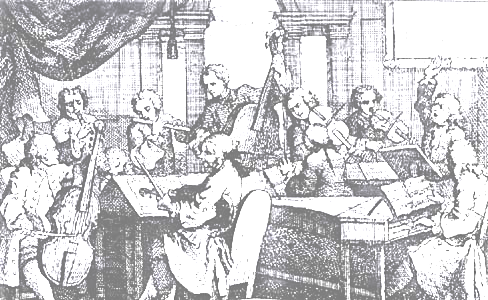
\includegraphics[scale=0.45]{../img/barocca.png}
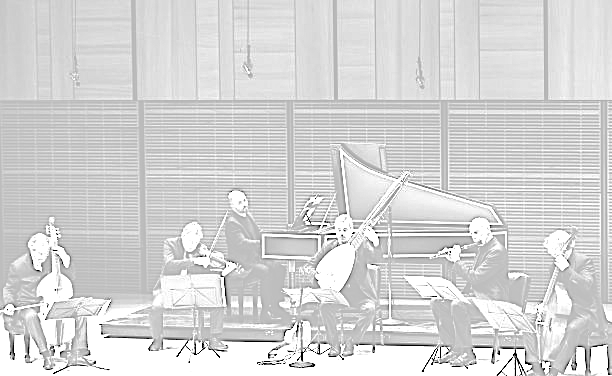
\includegraphics[scale=0.65]{../img/moderna.png}
\end{center}

The perception of a Beethoven symphony by an Amazonian native is totally different from ours, as is our perception of the microtones present in the \href{http://www.musicaecodice.it/gitmedia/emc/1_media/muezzin.mp3}{muezzin chants}.

\begin{center}

\includegraphics[scale=0.6]{../img/indigeni.png}
\end{center}

Let's also think about the technological dimension: the perception of the same sound text in a live concert is different from the perception of its reproduction recorded by an electroacoustic system perhaps while we wait for the subway.

\begin{center}
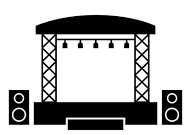
\includegraphics[scale=0.5]{../img/acousma.png}

\includegraphics[scale=0.5]{../img/sony.png}
\end{center}

\subsection{The work itself}\label{the-work-itself}

Regarding the understanding of the sound text itself Nattiez advocates the need to analyze: 

\begin{itemize}
\tightlist
\item works and styles as cultural and anthropological objects. 
\item harmony, rhythm, meter and all aspects that have a similar function in the grammar of natural language (comparison).
\end{itemize}

When we speak of grammars of musical parameters we are not referring exclusively to the analysis of the formal and structural characteristics of a specific musical text. We must also take into consideration the grammars of musical parameters generalized and historicized in styles and forms.

\begin{center}
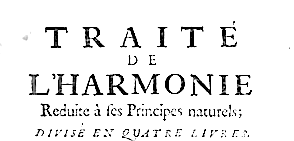
\includegraphics[scale=0.45]{../img/trattato.png}
\end{center}

Nattiez borrows from the study of verbal language the semantic exercise of breaking down meaning according to the use of words, which in music corresponds to the analysis of a melodic profile or a rhythmic system, or the distribution of harmonic fields in a tonal system or twelve-tone series, etc.

\begin{center}
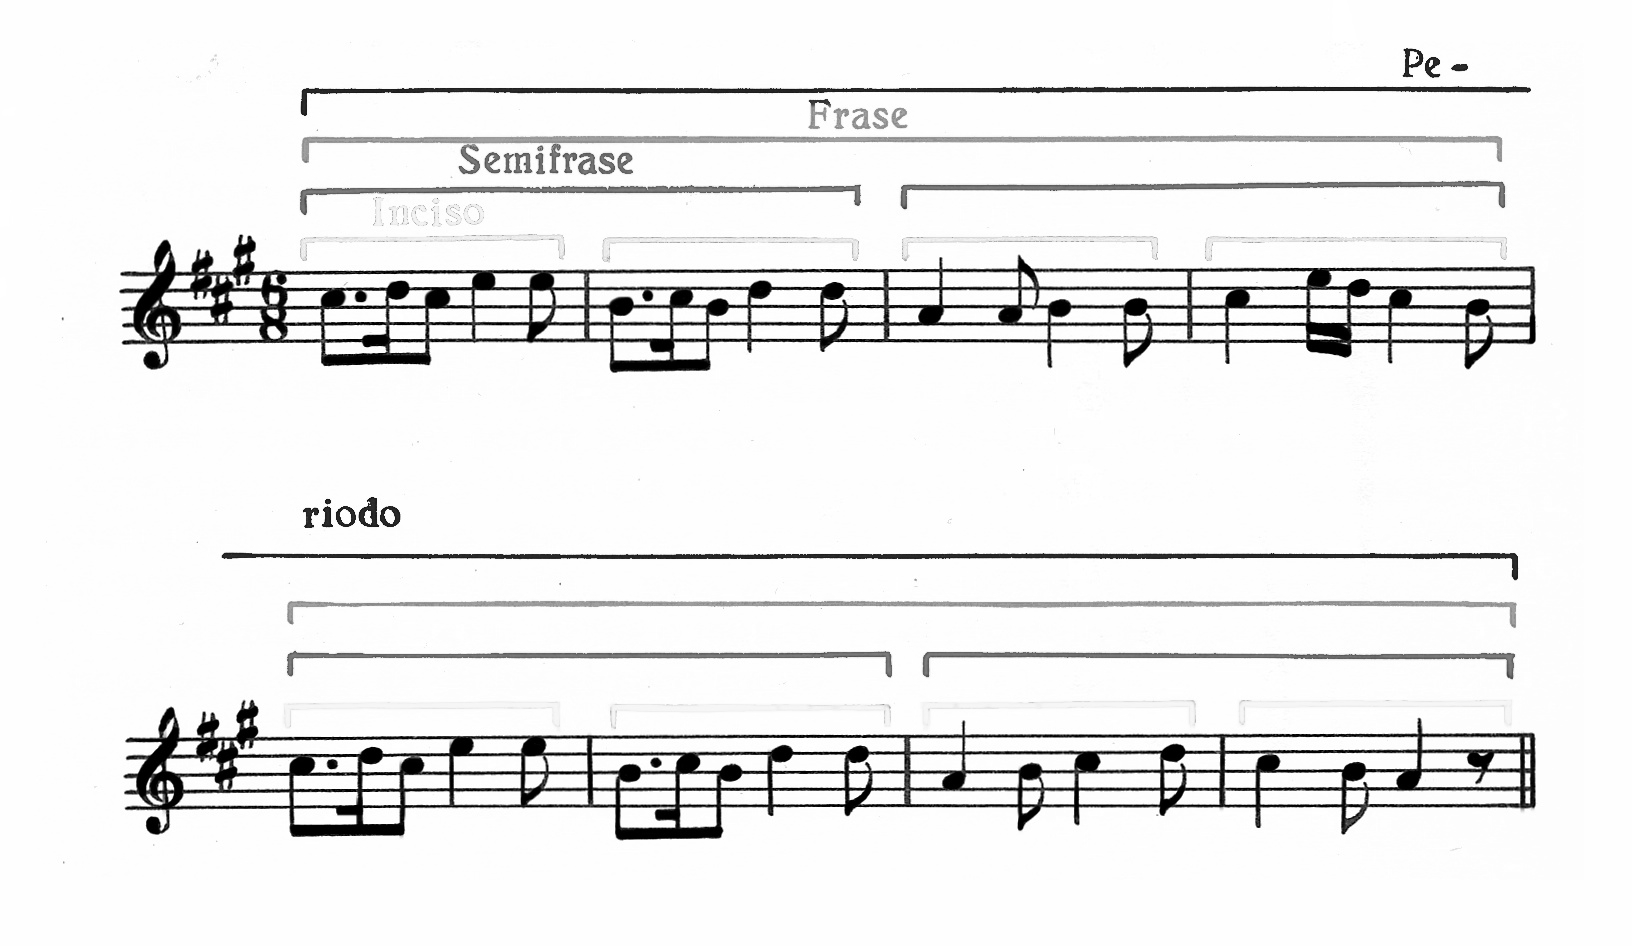
\includegraphics[scale=0.85]{../img/frasemus.png}
\end{center}

Each musical element (pitch, intensity, duration, timbre) can be separated and taken as a strategic variable in the production of a \href{http://www.musicaecodice.it/gitmedia/emc/1_media/quinta.mp4}{musical work}.

Ending, for Nattiez constructing a musical theory is the organization of a selection of interpretants adopted within an anthropological context.

Anyone who wants to invent a new musical grammar (a practice that has been widespread among art music composers since the 1950s) must take this into account and not just the definition of rules internal to the text.

Works do not exist in isolation since it is their place in history that provides their meaning and possible interpretations over time.

\begin{center}
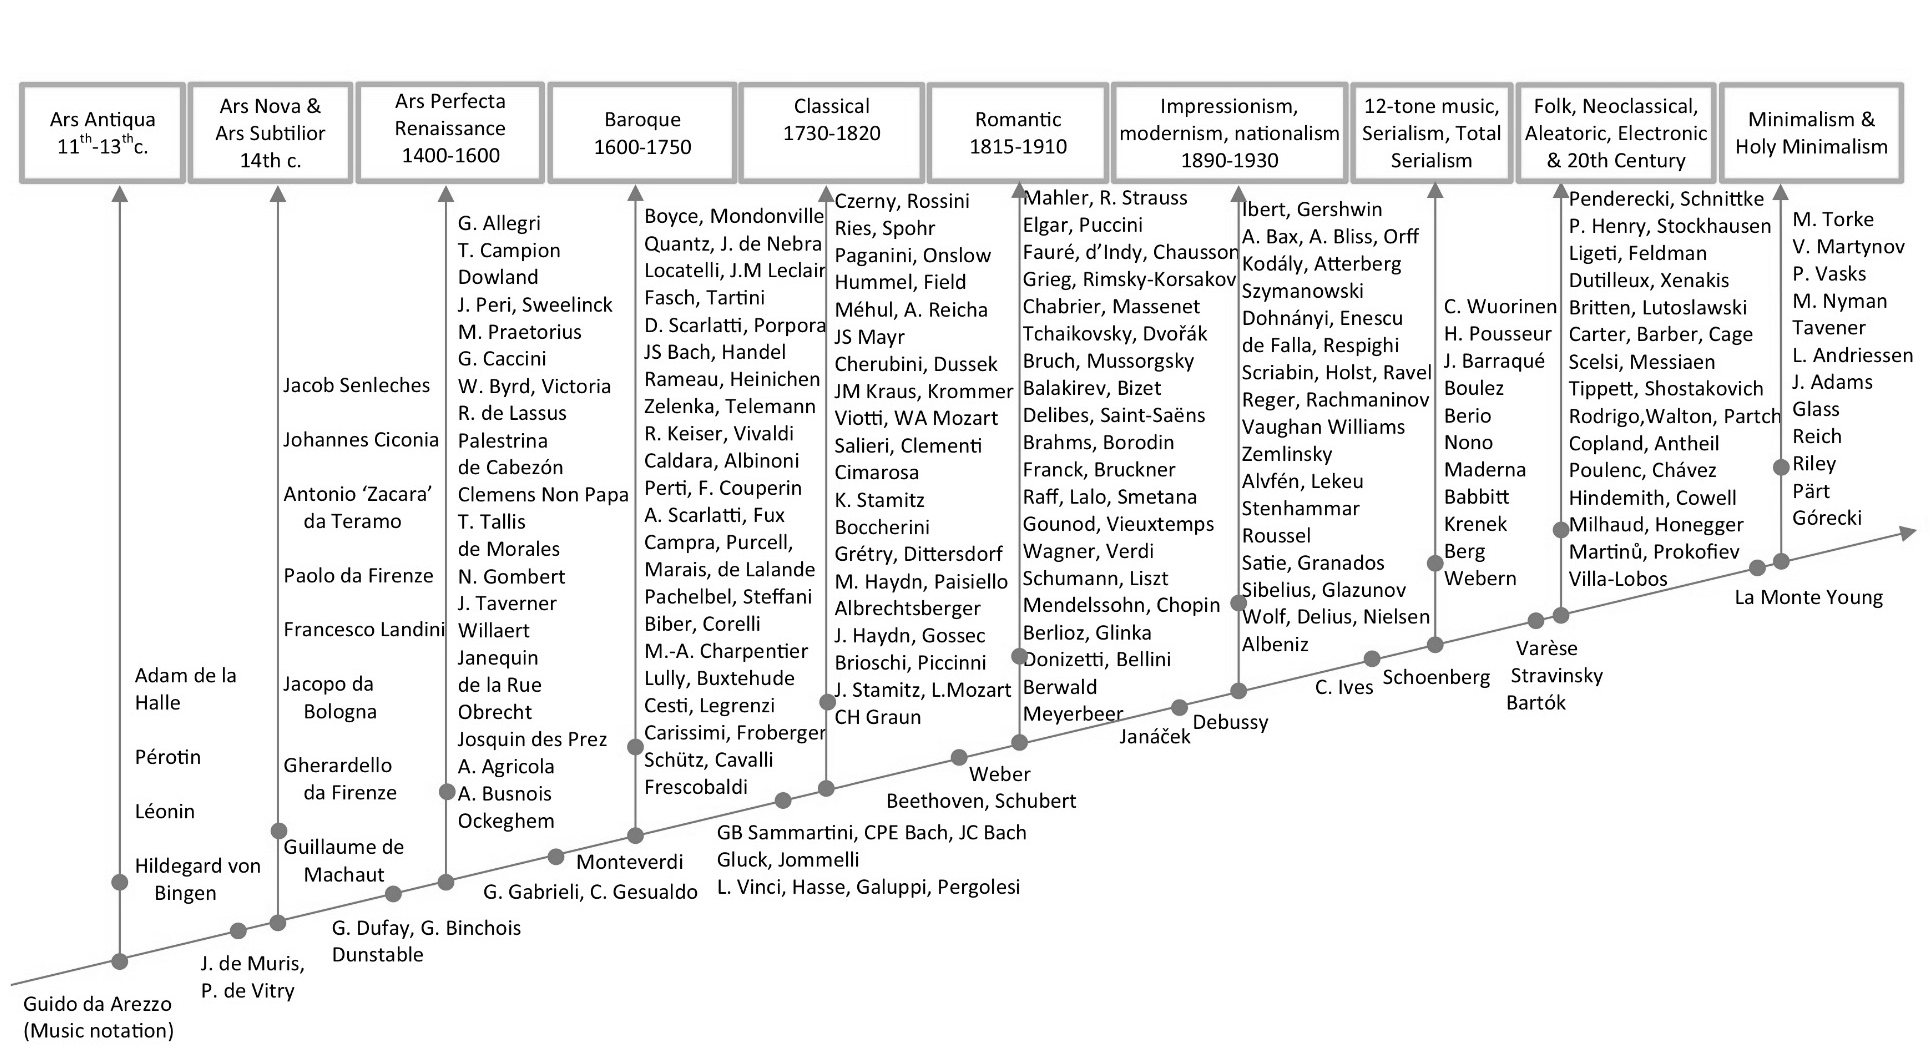
\includegraphics[scale=1]{../img/lineatempo.png}
\end{center}

The sound text can live a life of its own and be isolated from the the emitter but not from the anthropological context in which it was created and/or reproduced.

\subsection{Final reflections}\label{final-reflections}

Everyday life is filled with more or less voluntary signification.

Signification is the amniotic fluid within which human beings live.

We can highlight it and clarify its mechanisms.

This task is often hidden in everyday life.

For example, if we ask someone why they like a piece of music or a dress they will probably answer:

\begin{itemize}
\tightlist
\item because it's beautiful.
\item because it excites me.
\item because it's right.
\item because\ldots{}
\end{itemize}

Meaning often hides behind other motivations that tend to suppress it.

Let's think about written and spoken language.

In using it, we put into practice extremely complex knowledge that we tend to be unable to explain.

We would hardly be able to fully explain all the grammatical, phonetic, morphological, and syntactic rules we apply daily.

Language is practical knowledge that we almost never reason about (unless we are professional linguists).

Our daily experience works the same way: it appears random, spontaneous, and immediate.

In reality it is based on a dense and constantly changing network of relationships between things, people, places, etc.

Also the act of composing a piece of music should develops in the continuous passage from awareness of linguistic mechanisms (intelligence) to creativity.

Let'see a \href{http://www.musicaecodice.it/gitmedia/emc/1_media/senso1.mp4}{video}.
\chapter{Genres, instruments and tools}

\section{Genres}\label{genres}

Before starting to write an electroacoustic piece we should:

\begin{itemize}
\tightlist
\item define the instrumentation to be used which can include acoustic instruments, electroacoustic instruments, virtual instruments or a mix of these types.
\item define the sound amplification and diffusion system.
\end{itemize}

%\begin{center}
%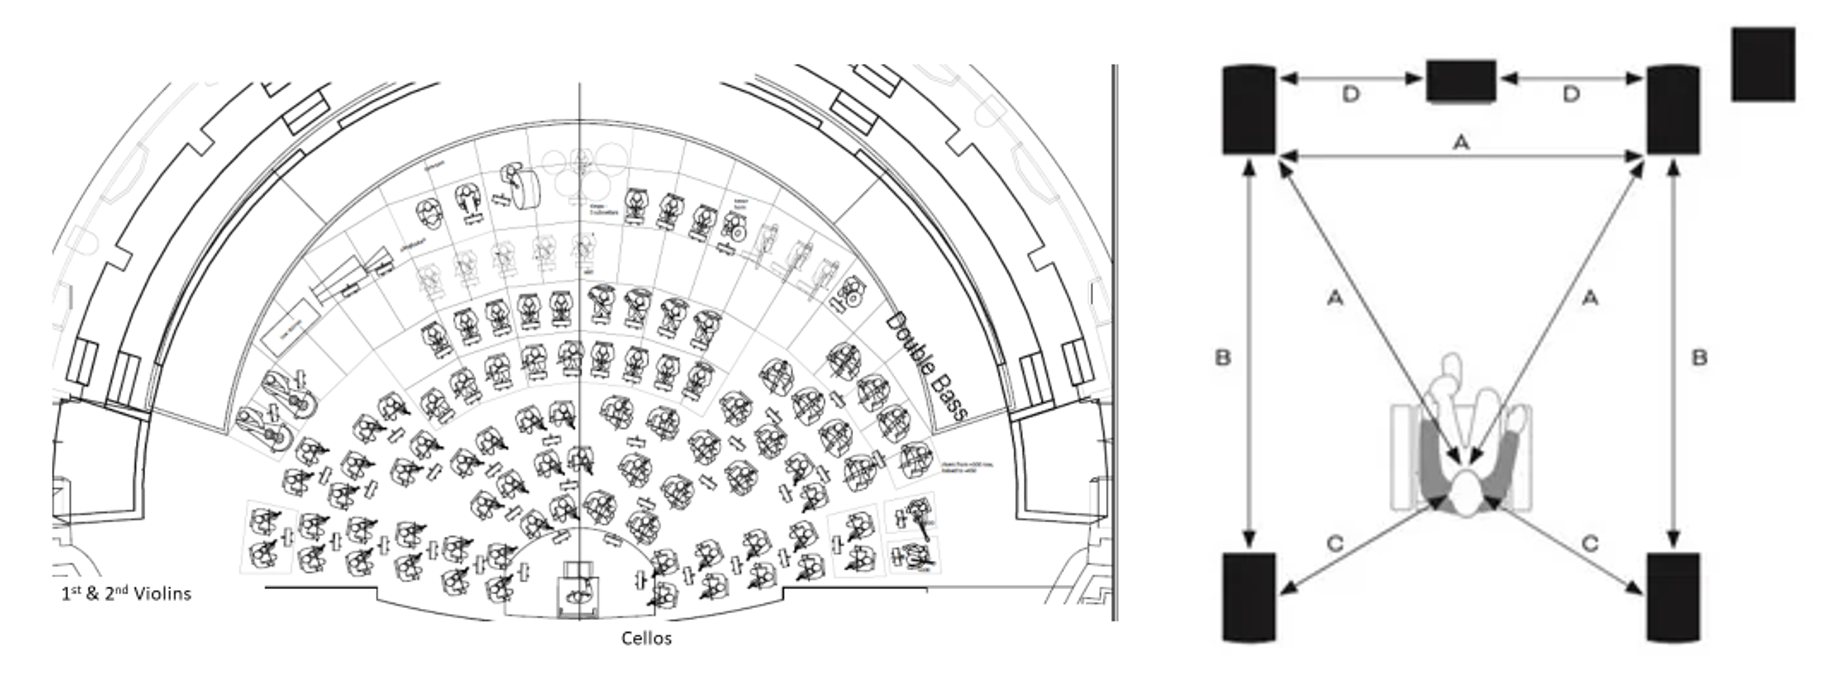
\includegraphics[scale=0.9]{img/dispo.png}
%\end{center}

For this reason here we categorize the different types and genres of electroacoustic music by dividing them into two macro areas defined by the way of controlling sounds and musical parameters.

\begin{itemize}
\tightlist
\item non interactive systems.
\item interactive systems.
\end{itemize}

We will explore the compositional strategies of each in dedicated chapters.

\section{Non interactive systems}\label{non-interactive-systems}

This category includes genres that:

\begin{itemize}
\tightlist
\item don't involve any human interaction during the performance.
\item involve interactions that don't influence the musical or sound text in any way.
\end{itemize}

According with the reflections of the previous chapter we can affirm:

\begin{itemize}
\tightlist
\item interactions may influence the listener's perception of the sound text (mainly through the different characteristics of the diffusion systems used).
\item interactions don't change the sound text.
\end{itemize}

This category can be divided into two further subcategories:

\begin{itemize}
\tightlist
\item fixed media music.
\item live sequencing.
\end{itemize}

The image shows the possibles audio chains in this category.

\begin{itemize}
\tightlist
\item non-real-time sound processing.
\item non-real-time synthesis.
\item real-time synthesis.
\end{itemize}

\begin{center}
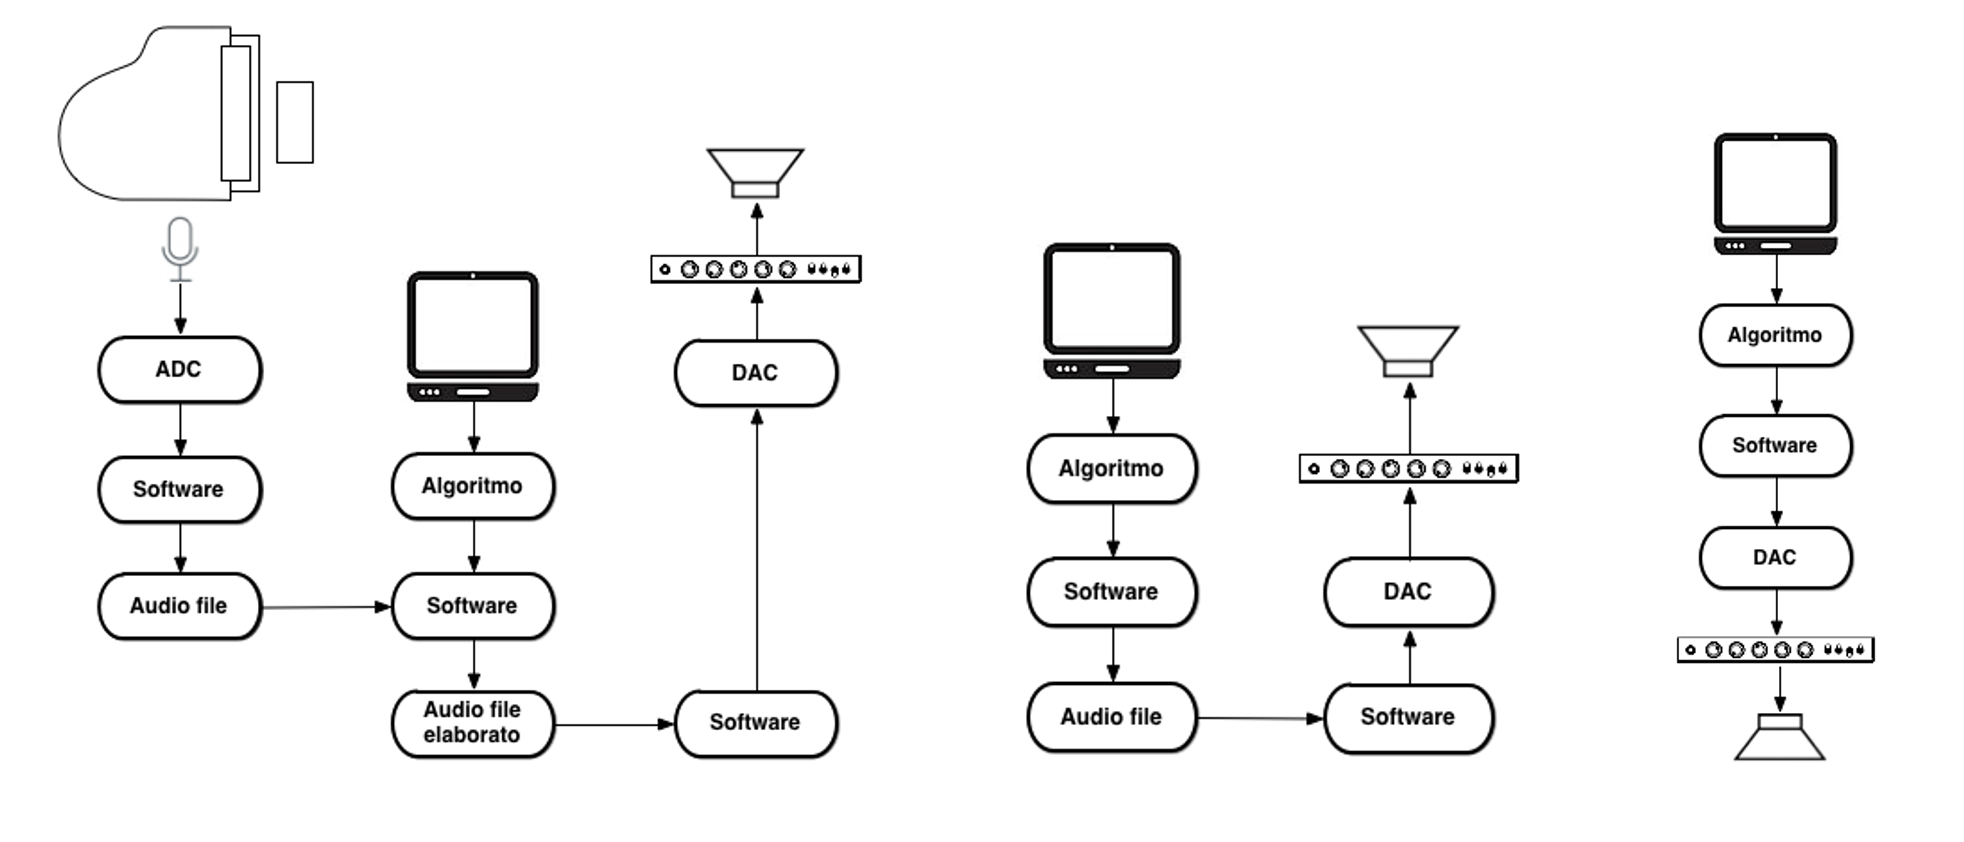
\includegraphics[scale=1]{../img/chains.png}
\end{center}

\subsection{Fixed media music }\label{fixed-media-music}

This subcategory denotes music or video that is played back from a recording.

This used to be called `tape music' but tapes are no longer used.

The entire work is stored on a single medium and reproduced from beginning to end.

We can identify three main genres:

\begin{itemize}
\tightlist
\item acousmatic music.
\item wallpaper music, ambient music and soundscapes.
\item radiodrama.
\end{itemize}

\subsubsection{Acousmatic music }\label{acousmatic-music}

\begin{center}
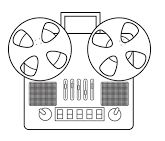
\includegraphics[scale=0.5]{../img/tape.png}
\end{center}

We can start from \textit{musique concrète}.

In the 1940s Pierre Schaeffer began composing with the sound (acoustic world).

After applying various sound elaborations (editing, filtering, reversal, etc.) he began to apply musical techniques to their combinations (repetition, transposition, reordering, etc.) inventing new musical structures (symbolic world).

In doing so, he reversed the compositional practice that had been in force for centuries in the Western musical tradition.

The listeners could not make the cognitive associations illustrated in the first chapter.

They activating exclusively the basic cognitive mechanisms common to all human beings.

This listening mode has been called \textit{reduced listening}.

All listeners of this new music are comparable to the aborigine who listens to a Beethoven symphony.

P.Shaeffer - \href{http://www.musicaecodice.it/gitmedia/emc/2_media/shaeffer.mp3}{Etude aux chemins de fer} for tape (1948) - extract.

\begin{itemize}
\tightlist
\item mono analog tape.
\item recorded and processed train sounds.
\item sounds from the acoustic environment.
\item we can recognize the sound source and its processing.
\item perceived as a distortion of reality.
\end{itemize}

Acousmatic music is the modern evolution of musique concrète.

By the mid-1970s a number of composers felt a need to designate their conception clearly in terms of specific methodology, syntax, and tools.

François Bayle suggested adopting the term acousmatique.

This term comes from the Greekakousma: what is heard.

Students of Pythagoras listened to his teachings from behind a screen unable to see him.

He believed that the lack of visual cues would force his students to focus all their attention on his message.

After his death his followers split into:

\begin{itemize}
\tightlist
\item acousmatics (practitioners of the mystic doctrine)
\item mathematics (scientists).
\end{itemize}

The loudspeaker was the modern equivalent of the screen partition.

\textit{"From an esthetical point of view acousmatic music concentrates on the poetical and spectral richness of sounds, and plays with this very particular characteristic of sound hearing in which the perception of anacoustic phenomena is associated with its cause; hence the perception of a sound whose cause is unknown or unrecognizable for our perception, induces the listener to imagine non-existing causes and to perceive
music as a complex creative phenomena in which musical sense and musical sounds have to be interpreted simultaneously, with generally very little relation with our perceptive reality. The question is not to find out how sounds are made but how their combination will generate imaginary perceptions of imaginary realities in our mind."}

Teruggi, D. 1995. What about acousmatics? In Journal of Electroacoustic
Music. Vol. 7. London: Sonic Arts Network

\href{http://www.musicaecodice.it/gitmedia/emc/2_media/teruggi.pdf}{More info}

B.Parmegiani - \href{http://www.musicaecodice.it/gitmedia/emc/2_media/parmegiani.mp3}{De Natura Sonorum} for tape (1975) - extract.

\begin{itemize}
\tightlist
\item stereo digital tape.
\item recorded and processed sounds plus synthetic sounds.
\item sounds from an imaginary environment.
\item we cannot recognize the sound source.
\item perceived as an alternative or virtual reality.
\end{itemize}

Another characteristic of acousmatic music is that it is performed live on loudspeaker orchestras (acousmonium).

Indeed Bayle referred to acousmatic musica as \textit{"art of projected sounds which is shot and developed in the studio, projected in a hall, like cinema".}

H.Vaggione - \href{http://www.musicaecodice.it/gitmedia/emc/2_media/vaggione.mp3}{Consort}. for convolved violins (2011) - extract.

\begin{itemize}
\tightlist
\item multitrack digital file.
\item recorded and processed instrumental sounds.
\item sounds from music environment.
\item we can recognize the sound source and its avatars.
\item perceived as a piece of music.
\end{itemize}

\href{http://www.musicaecodice.it/gitmedia/emc/2_media/space.pdf}{More info} about acousmatic works interpretation.

\subsubsection{Wallpaper music, ambient music and soundscapes }\label{wallpaper-music-ambient-music-and-soundscapes}

\begin{center}

\includegraphics[scale=0.4]{../img/ambi.png}
\end{center}

We can start from Eric Satie (non-electroacoustic composer).

He was a precursor of minimalism, muzak, and many other 20th-century musical genres.

Satie conceived this musical genre as a backdrop to everyday activities (passive listening).

Satie was familiar with this idea due to its role as role as a Montmartre café pianist in the late 19th and early 20th century.

E.Satie - \href{http://www.musicaecodice.it/gitmedia/emc/2_media/satie.mp3}{Musique d'ameublement} (1917) for ensemble - extract.

\begin{itemize}
\tightlist
\item acoustic instruments.
\item pattern iteration.
\item music environment.
\item time dilation (psychological time).
\item passive and non immersive listening.
\item perceived as a piece of music.
\end{itemize}

We know well how nowadays we are bombarded daily by this type of music in a totally involuntary motion.

Let us recall what was stated in the first chapter on the basic cognitive mechanisms of human beings.

In the 1950s a visionary composer like J.Cage took this idea to its extreme with the piece 4'33'\,' whose sonic and musical content consists of the background noise of a finite time.

Later in 1978 another composer Brian Eno coined the term ambient as a musical genre.

A Sunday morning in the Cologne airport while waiting for a flight he tought: \textit{The light was beautiful, everything was beautiful, except they were playing awful music. They spend hundreds of millions of pounds\ldots on everything. Except the music.}

It was this that compelled him to begin composing music for public environments.

We must consider that the diffusion of sounds and/or music in environments not designed for active listening can change the perception of that environment in a subconscious way.

It is time that through sound redraws the boundaries of a space.

B.Eno - \href{http://www.musicaecodice.it/gitmedia/emc/2_media/eno.mp3}{Music for Airports} (1978) for tape - extract.

\begin{itemize}
\tightlist
\item stereo vynil. 
\item pattern iteration.
\item music environment. 
\item time dilation (psychological time). 
\item passive and semi immersive listening. 
\item perceived as a piece of music.
\end{itemize}

\href{http://www.musicaecodice.it/gitmedia/emc/2_media/eno.pdf}{More info}

Soundscape composition can represent a meeting point between musique concrete and ambient music because:

\begin{itemize}
\tightlist
\item it uses sound materials recorded from the real world or synthesized.
\item does not recompose them according to symbolic rules and principles into a musical form.
\item its purpose is to construct or reconstruct a real or virtual soundscape.
\end{itemize}

It's essentially based on the studies and works of Canadian musicologist and composer Raymond Murray Schafer.

To put it simply, we can say that different types of sounds coexist in a sound environment and we can identify three types:

\begin{itemize}
\tightlist
\item geophony \(\rightarrow\) all the sounds of nature of non-biological origin.
\item biophony \(\rightarrow\) all the sounds of nature of biological origin but not caused by humans.
\item anthrophony \(\rightarrow\) all sounds generated by humans.
  \begin{itemize}
  \tightlist
  \item language.
  \item music.
  \item mechanical sound.
  \end{itemize}
\end{itemize}

Schafer also divides the sounds of a soundscape into two categories:

\begin{itemize}
\tightlist
\item hi-fi \(\rightarrow\) all sounds that have an hight signal-to-noise ratio (they are distinguishable from the background noise).
\item lo-fi \(\rightarrow\) all sounds that have a low signal-to-noise ratio (they are indistinguishable from the background noise).
\end{itemize}

Three main elements in a soundscape:

\begin{itemize}
\tightlist
\item keynote \(\rightarrow\) sounds that most characterize an environment, analogous to the tonality in tonal music.
\item sound signals \(\rightarrow\) all the foreground sounds that do not necessarily characterize an environment but may appear occasionally.
\item soundmark \(\rightarrow\) The unique sounds of a given soundscape.
\end{itemize}

N.Barret - \href{http://www.musicaecodice.it/gitmedia/emc/2_media/soundwalk.mp3}{Soundwalk} (1998) - extract.

\begin{itemize}
\tightlist
\item stereo digital tape. 
\item no pattern. 
\item acoustic environment. 
\item time as in real life (clock time). 
\item passive and immersive listening. 
\item perceived as an acoustoc environment.
\end{itemize}

\href{http://www.musicaecodice.it/gitmedia/emc/2_media//schafer.pdf}{More info}

\subsubsection{Radiodrama }\label{radiodrama}

\begin{center}

\includegraphics[scale=0.5]{../img/radio.png}
\end{center}

Radio drama can use only four kinds of signs:

\begin{itemize}
\tightlist
\item speech.
\item sound effects.
\item music.
\item silence.
\end{itemize}

Any one of these by itself can be a very slippery client to deal with.

Silence cane a listener suspect a transmission failure and switch off or tune over to another on.

Sound effects are notoriously misleading - a sneeze can be taken for a bomb explosion!

An unfamiliar music will sound irritatingly like cacophony.

And speech says nothing to someone who doesn't know what you mean by the words.

But if you hit on harmonious combination of the right choies of these four kinds you can move mountains, deploy infantry battalions with Air Force support, immerse a soul in the joys of paradise.

In short do anything you please, all in few minutes one after another.

The main focus is narrativity and a continuous balance in the construction of meaning between explicit sounds (both in natural and auditory language) and perceptual hints and/or allusions.

O.Wells - \href{http://www.musicaecodice.it/gitmedia/emc/2_media/wells.mp3}{War of the worlds} (1938) - extract.

\begin{itemize}
\tightlist
\item mono radio signal.
\item natural language.
\item didactic sound design to simulate the real acoustic environment.
\item time as in real life (clock time).
\item active listening non immersive.
\item perceived as a representation of reality.
\end{itemize}

\href{http://www.musicaecodice.it/gitmedia/emc/2_media/radio.pdf}{More info}

\subsubsection{Computer music - algorithmic composition}\label{computer-music---algorithmic-composition}

\begin{center}

\includegraphics[scale=0.5]{../img/comp.png}
\end{center}

The birth of computer music is naturally linked to the invention of the electronic calculator and the subsequent spread of personal computers as well as the invention of new (formal) languages that allow humans to communicate with these machines.

Starting from the second half of the 1950s, two orientations emerged:

\begin{itemize}
\tightlist
\item the first one (developed mainly in Europe) deals with the digital coding of musical parameters (assisted composition, assisted musical analysis, etc.).
\item the second one (developed mainly in USA) deals with the digital coding of sound parameters (synthesis and processing).
\end{itemize}

In 1957 MUSIC I was created by Max Mathews in Bell Laboratories.

It was the first software for playing music from mathematical functions.

After MUSIC I, there were: MUSIC II, III, IV, V, MUSIC 360, and then C-sound and SuperCollider languages still used today.

The main sound synthesis and processing techniques used are:

\begin{itemize}
\tightlist
\item additive synthesis.
\item subctractive synthesis (filters).
\item FM (Frequency Modulation) synthesis.
\item granular synthesis.
\item analysis and resynthesis (FFT).
\item generative algorithms for:

  \begin{itemize} 
  \tightlist
  \item musical structures.
  \item timbres.
  \item pitches.
  \end{itemize}
\item remote control of computers (MIDI, OSC, HID).
\end{itemize}

As we all know, nowadays computer is the main musical instrument, like piano in the 19th century.

The term \textit{computer music} as an aesthetic category identifies the musical genre adopted by the pioneers from the mid-50s to the late 90s

J.Chowning - \href{http://www.musicaecodice.it/gitmedia/emc/2_media/chowning%20.mp3}{Stria}. (1977) - extract.

\begin{itemize}
\tightlist
\item stereo digital tape.
\item sonic environment.
\item sounds from imaginary environment (only synthetic sounds - FM).
\item time dilation (psychological time).
\item active listening.
\item perceived as a piece of computer music.
\end{itemize}

\href{http://www.musicaecodice.it/gitmedia/emc/2_media/max.pdf}{More info}

\subsection{Live sequencing}\label{live-sequencing}

This subcategory is almost identical to the previous one except for two aspects: 

\begin{itemize}
\tightlist
\item works can be generated in real time through algorithms (computer music). 
\item tracks are divided into different sound files triggered in real time (sound design for theatre and gaming).
\end{itemize}

\subsubsection{Sound design for performing arts or video }\label{sound-design-for-performing-arts-or-video}

\begin{center}
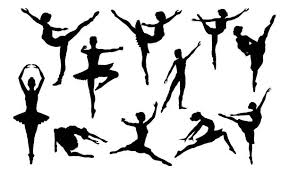
\includegraphics[scale=0.4]{../img/danza.png}
\end{center}

Works on fixed media which differ from the works illustrated in the previous section essentially for:

\begin{itemize}
\tightlist
\item sound does not have an absolute value but must be functional to dramaturgy.
\item divised into more or less short fragments.
\item open form \(\rightarrow\) fragments can be triggered in non-linear sequences (slightly different than what was said about random generation).
\item differenze musicali rispetto ai brani acusmatici.
\end{itemize}

Anonymous - \href{http://www.musicaecodice.it/gitmedia/emc/2_media/dance.mp3}{Dance!} (2010) - extract.

\begin{itemize}
\tightlist 
\item stereo digital tape. 
\item music functional to movement or dramatic timing.
\item secondary sensitive plane. 
\item passive listening. 
\item perceived as a complement to visual information.
\end{itemize}

\subsubsection{Sound design for gaming}\label{sound-design-for-gaming}

\begin{center}

\includegraphics[scale=0.3]{../img/game.png}
\end{center}

In this case too the sound must be functional to the game

It should:

\begin{itemize}
\tightlist
\item suggest a mood, evoke a feeling.
\item indicate a geographical locale.
\item define a character.
\item mirror or exaggerate how things sound in real life.
\item clarify the narrative
\end{itemize}

To simplify there are five sounds categories:

\begin{itemize}
\tightlist
\item dialogue \(\rightarrow\) any verbal speech in the game (player talk).
\item music \(\rightarrow\) any non-diegetic music (orchestral music).
\item sound Effects (Hard Effects) \(\rightarrow\) any sound from an real-life object (sounds of rocks falling).
\item foley \(\rightarrow\) any sound effect that the player makes (footsteps, etc.).
\item backgrounds (ambience) \(\rightarrow\) noise from the environment (wind, rain, etc.).
\end{itemize}

Procedural audio:

\begin{itemize}
\tightlist
\item sounfiles triggered by user actions.
\item real time shynthesis by internal oscillators.
\end{itemize}

Artistically we could merge game music, soundscape composition, acousmatic music and radiodrama.

Various - \href{http://www.musicaecodice.it/gitmedia/emc/2_media/gaming.mp3}{8 bit music}(1990) - extracts.

\begin{itemize}
\tightlist
\item stereo digital samples or real time oscillators.
\item music functional to gamer emotions.
\item also called procedural music.
\item pattern iteration.
\item music environment.
\item time dilation (psychological time).
\item non-immersive audio diffusion but immersive psychological function.
\item passive listening.
\end{itemize}

\href{http://www.musicaecodice.it/gitmedia/emc/2_media/gaming.pdf}{More info}

\section{Interactive systems }\label{interactive-systems}

This category includes genres that:

\begin{itemize}
\tightlist
\item involve human interaction during the performance as happens with acoustic instruments.
\item these interactions influence the musical or sound text at different levels.
\end{itemize}

Compared to the previous typology the presence of one or more performers significantly influences:

\begin{itemize}
\tightlist
\item the anthropological and contextualised perception of the musical action.
\item its representative nature.
\end{itemize}

This category can be divided into three further subcategories:

\begin{itemize}
\tightlist
\item hyper-instruments.
\item live set.
\item live coding.
\end{itemize}

The image shows the possibles audio chains in this category.

\begin{itemize}
\tightlist
\item real-time processing of pre-recorded or pre-synthesized sounds (parameters can be controlled through various types of devices - MIDI, OSC, HID, sensors).
\item real-time processing of signals captured through microphones or sensors (parameters can be controlled (parameters can be controlled in the previous modes but also through control signals derived in some way from the incoming audio signal).
\end{itemize}

\begin{center}
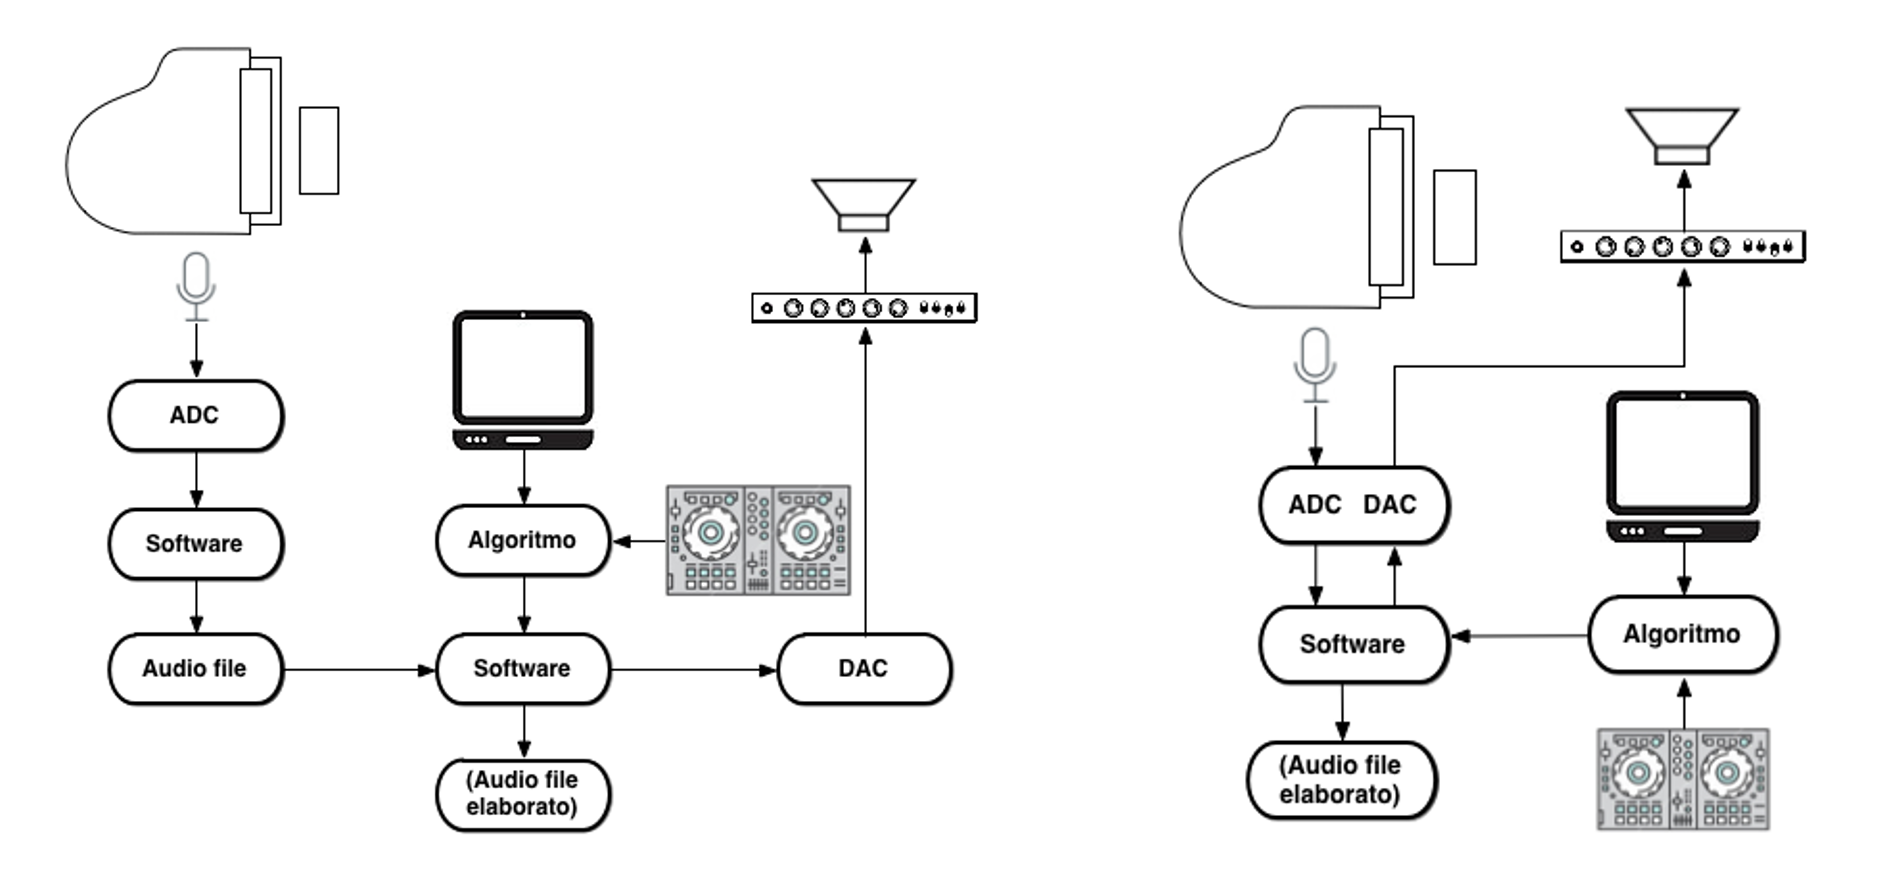
\includegraphics[scale=1]{../img/chain2.png}
\end{center}

\subsection{Hyper-instrument}\label{hyper-instrument}

\begin{center}

\includegraphics[scale=0.6]{../img/lel.png}\\
P.Boulez - \href{http://www.musicaecodice.it/gitmedia/emc/2_media/boulez1.mp4}{Anthèmes 2} (1994) - extract.
\end{center}

Augmented musical instrument that uses technology to extend the capabilities of a traditional instrument and enhance the performer's expressiveness.

Two types:

\begin{itemize}
\tightlist
\item real-time augmented instrumental techniques \(\rightarrow\) sound processes are controlled by:

  \begin{itemize}
  \tightlist
  \item an electronic performer who interacts with different types of controllers.
  \item by information extracted from the audio signal produced by the instrument itself (feature extraction as control signals).
  \end{itemize}
\item cyborg luthiery \(\rightarrow\) sound processing is controlled by movements and/or gestures of the performer captured by different types of sensors.
\end{itemize}

Three main goals:

\begin{itemize}
\tightlist
\item respond to the performer's input in a dynamic and expressive way allowing for a deeper connection between the musician and the music.
\item produce sounds and musical effects that are impossible to achieve with traditional instruments alone.
\item expanding musical forms.
\end{itemize}

\subsection{Live set }\label{live-set}

\begin{center}
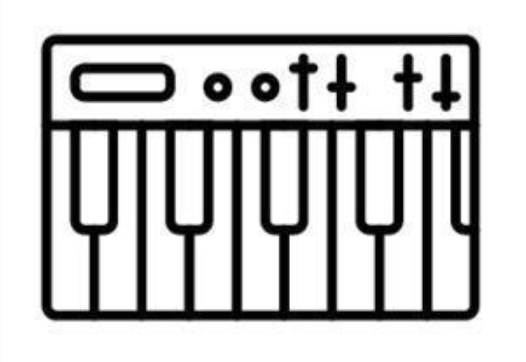
\includegraphics[scale=0.3]{../img/lset.png}\\
Slork - \href{http://www.musicaecodice.it/gitmedia/emc/2_media/slork1.mp4}{Twilight} (2013) - extract.
\end{center}

Live performance where songs are performed using analog or digital electronic musical instruments.

Often musicians improvise in a live set, making each performance unique.

Can be a solo performance or a laptop ensemble.

One of the most important aspects of this genre is to think about and assemble original performance environments which leads to the search for new human/machine interfaces dedicated to the generation of new sounds in the musical field.

\subsection{Live coding}\label{live-coding}

\begin{center}

\includegraphics[scale=0.4]{../img/lcod.png}\\
SuperCollider \href{http://www.musicaecodice.it/gitmedia/emc/2_media/livec1.mp4}{Live Coding} - extract.
\end{center}

Also called:

\begin{itemize}
\tightlist
\item on-the-fly programming.
\item just in time programming.
\item conversational programming.
\end{itemize}

Search for new musical forms, new places for performance and new audiences.

It is part of a larger artistic movement called creative coding.

If channeled into the Western musical tradition, we can think of it as a new version of organ improvisations in the Baroque era.

From a semiographic point of view the most interesting aspect is that the score is the code and is created and manipulated in real time.

The compositional process which has always belonged to the author's private sphere becomes public and an integral part of the performance itself (do you remember the first paragraphs of the previous chapter?).

\section{The virtual instrument paradigm}\label{the-virtual-instrument-paradigm}

In this section we define a virtual instrument model that will be useful in next chapters.

If anyone is unfamiliar with SuperCollider, they can download an introductory text at
\href{https://ccrma.stanford.edu/~ruviaro/texts/A_Gentle_Introduction_To_SuperCollider.pdf}{this
link}.

In the chapter on live electronics we'll make some small modifications to allow signal input.

\subsection{Software installation }\label{software-installation}

Download and install:

\begin{itemize}
\tightlist
\item \href{https://github.com/capital-G/sc_kernel}{sc\_kernel} (if you want to execute supercollider code in this notebook)
\item \href{https://supercollider.github.io/}{SuperCollider}
\end{itemize}

If you want to play SuperCollider from this notebook you have to select the textit{sc\_kernel}.

Instead, I recommend copying and pasting the code into the SuperCollider IDE Interpreter.

\subsection{Instrumental model}\label{instrumental-model}

Let's create a computer model that contains functions common to most virtual instruments (sound generators).

\begin{itemize}
\tightlist
\item an oscillator.
\item an amplitude envelope (with or without sustain).
\item a stereo panner.
\item a signal output.
\end{itemize}

We also establish the basic parameters we want to control dynamically (they will increase depending on the synthesis algorithm chosen).

\begin{itemize}
\tightlist
\item frequency (Hz).
\item general amplitude (0.0 to 1.0).
\item duration (seconds).
\item pan position (-1.0 to +1-0).
\item pan interpolation time (movements)
\item output bus.
\item trigger.
\item kind of voice allocation (doneAction:0 or 2).
\end{itemize}

\begin{center}
\includegraphics[scale=0.35]{../img/modello.png}
\end{center}

\begin{lstlisting}[frame=single] 
s.boot;
s.meter;
s.scope;
s.plotTree;
\end{lstlisting}

In SuperCollider we can define it with the `SynthDef' (synthesis definition) class.

This class contains the instructions (algorithms) needed to build multiple copies (instances) derived from the model.

\begin{lstlisting}[frame=single, caption=Instrument model] 
SynthDef.new(\model, {arg freq=500, amp=0, dur=1, pan=0, pantime(0.0), 
                          out=0, t_gate=0, done=2;
                      var sig, env;
                          sig = SinOsc.ar(freq);
                          env = Env.new([0.0,1.0,0.5,0.7,0],                
                                        [0.1,0.1,0.3,1.0].normalizeSum * dur,
                                        -4    
                                        );
                          env = EnvGen.kr(env, t_gate, doneAction:done);
                          sig = sig * env * amp;
                          sig = Pan2.ar(sig, pan.varlag(pantime));
                      Out.ar(out, sig)
                      }).add;        
\end{lstlisting}
Now we can generate as many instances as we want.

We have two ways to control the instance parameters.

They vary depending on the voice allocation we want.

\textbf{Dynamic voice allocation (poliphonic)} 

Instance self-destructs when the amplitude envelope expires (doneAction:2).

In this case we pass parameters at instantiation time (array of \textbackslash key, value).

\begin{lstlisting}[frame=single,caption=Dynamic voice allocation] 
Synth.new(\model, [\freq, rrand(890,1234), 
                   \amp, 0.5, 
                   \dur, rrand(0.1,2), 
                   \pan, rand2(1.0), 
                   \pantime, 0.1, 
                   \done, 2, 
                   \t_gate,1 ])
\end{lstlisting}

\textbf{Static voice allocation (monophnic)}

Two passages: 

\begin{itemize}
\tightlist
\item create instance and assign it to a variable.
\item send one or multiple parameter changes by \textit{set} method.

\begin{lstlisting}[frame=single, caption=Static voice allocation] 
a = Synth.new(\model, [\done, 0]);
a.set(\freq, rrand(890,1234), 
      \amp, 0.5, 
      \dur, rrand(0.1,2), 
      \pan, rand2(1.0), 
      \pantime, 0.1, 
      \t_gate,1)
\end{lstlisting}
\end{itemize}

Then we can kill it.

\begin{lstlisting}[frame=single] 
a.free;
\end{lstlisting}
Or kill all Synths on the Server.

\begin{lstlisting}[frame=single] 
s.freeAll;
\end{lstlisting}
The type of voice allocation is strictly linked to the type of amplitude envelope.

\textbf{With sustain (as in keyboards)}

There isn't a total duration.

In this case we must send a message of \textit{gate 1} (noteon) and then textit{gate 0} (noteoff).

\begin{lstlisting}[frame=single, caption=Instrument model with sustain] 
SynthDef.new(\sust, {arg freq=500, amp=0, pan=0, pantime(0.0), 
                     out=0, gate=0, done=2;
                     var sig, env;
                         sig = SinOsc.ar(freq);
                         env = Env.adsr;         
                         env = EnvGen.kr(env, gate, doneAction:done);
                         sig = sig * env * amp;
                         sig = Pan2.ar(sig, 0);
                     Out.ar(0, sig)
                     }).add;       
                                                
a = Synth.new(\sust, [\done, 0]); 
\end{lstlisting}
Send \textit{gate 1} (noteon)
\begin{lstlisting}[frame=single] 
a.set(\amp, 0.5, \gate, 1);
\end{lstlisting}
Send \textit{gate 0} (noteoff)
\begin{lstlisting}[frame=single] 
a.set(\gate, 0);
\end{lstlisting}
Kill the Synth.
\begin{lstlisting}[frame=single] 
a.free;
\end{lstlisting}

\textbf{Without sustain (as in percussion or plucked intruments)}

There is a total duration.

In this case we must send a gate message preceded by \textit{t\_}.

This produce an automatic \textit{gate 0} message after a time calculated on the specified duration

\begin{lstlisting}[frame=single, caption=Instrument model without sustain] 
SynthDef.new(\nosust,  {arg freq=500, amp=0, dur=1, pan=0, pantime(0.0), 
                            out=0, t_gate=0, done=2;
                        var sig, env;
                            sig = SinOsc.ar(freq);
                            env = Env.perc(0.1*dur,0.9*dur);                     
                            env = EnvGen.kr(env, t_gate, doneAction:done);
                            sig = sig * env * amp;
                            sig = Pan2.ar(sig, 0);
                        Out.ar(0, sig)
                        }).add;                                                   
a = Synth.new(\nosust, [\done, 0]);    // Create the Synth
\end{lstlisting}

Send \textit{t\_gate 1} (noteon + noteoff)

\begin{lstlisting}[frame=single] 
a.set(\amp, 0.5, \t_gate,1);
\end{lstlisting}

You can also trigger and kill it automatically.

\begin{lstlisting}[frame=single] 
a.set(\amp, 0.5, \done, 2, \t_gate,1);
\end{lstlisting}

Modifications to this model will be addressed in specific chapters.




\end{document}